\documentclass[twoside]{book}

% Packages required by doxygen
\usepackage{fixltx2e}
\usepackage{calc}
\usepackage{doxygen}
\usepackage[export]{adjustbox} % also loads graphicx
\usepackage{graphicx}
\usepackage[utf8]{inputenc}
\usepackage{makeidx}
\usepackage{multicol}
\usepackage{multirow}
\PassOptionsToPackage{warn}{textcomp}
\usepackage{textcomp}
\usepackage[nointegrals]{wasysym}
\usepackage[table]{xcolor}

% Font selection
\usepackage[T1]{fontenc}
\usepackage[scaled=.90]{helvet}
\usepackage{courier}
\usepackage{amssymb}
\usepackage{sectsty}
\renewcommand{\familydefault}{\sfdefault}
\allsectionsfont{%
  \fontseries{bc}\selectfont%
  \color{darkgray}%
}
\renewcommand{\DoxyLabelFont}{%
  \fontseries{bc}\selectfont%
  \color{darkgray}%
}
\newcommand{\+}{\discretionary{\mbox{\scriptsize$\hookleftarrow$}}{}{}}

% Page & text layout
\usepackage{geometry}
\geometry{%
  a4paper,%
  top=2.5cm,%
  bottom=2.5cm,%
  left=2.5cm,%
  right=2.5cm%
}
\tolerance=750
\hfuzz=15pt
\hbadness=750
\setlength{\emergencystretch}{15pt}
\setlength{\parindent}{0cm}
\setlength{\parskip}{0.2cm}
\makeatletter
\renewcommand{\paragraph}{%
  \@startsection{paragraph}{4}{0ex}{-1.0ex}{1.0ex}{%
    \normalfont\normalsize\bfseries\SS@parafont%
  }%
}
\renewcommand{\subparagraph}{%
  \@startsection{subparagraph}{5}{0ex}{-1.0ex}{1.0ex}{%
    \normalfont\normalsize\bfseries\SS@subparafont%
  }%
}
\makeatother

% Headers & footers
\usepackage{fancyhdr}
\pagestyle{fancyplain}
\fancyhead[LE]{\fancyplain{}{\bfseries\thepage}}
\fancyhead[CE]{\fancyplain{}{}}
\fancyhead[RE]{\fancyplain{}{\bfseries\leftmark}}
\fancyhead[LO]{\fancyplain{}{\bfseries\rightmark}}
\fancyhead[CO]{\fancyplain{}{}}
\fancyhead[RO]{\fancyplain{}{\bfseries\thepage}}
\fancyfoot[LE]{\fancyplain{}{}}
\fancyfoot[CE]{\fancyplain{}{}}
\fancyfoot[RE]{\fancyplain{}{\bfseries\scriptsize Generated on Thu Dec 3 2015 11\+:42\+:20 for My Project by Doxygen }}
\fancyfoot[LO]{\fancyplain{}{\bfseries\scriptsize Generated on Thu Dec 3 2015 11\+:42\+:20 for My Project by Doxygen }}
\fancyfoot[CO]{\fancyplain{}{}}
\fancyfoot[RO]{\fancyplain{}{}}
\renewcommand{\footrulewidth}{0.4pt}
\renewcommand{\chaptermark}[1]{%
  \markboth{#1}{}%
}
\renewcommand{\sectionmark}[1]{%
  \markright{\thesection\ #1}%
}

% Indices & bibliography
\usepackage{natbib}
\usepackage[titles]{tocloft}
\setcounter{tocdepth}{3}
\setcounter{secnumdepth}{5}
\makeindex

% Hyperlinks (required, but should be loaded last)
\usepackage{ifpdf}
\ifpdf
  \usepackage[pdftex,pagebackref=true]{hyperref}
\else
  \usepackage[ps2pdf,pagebackref=true]{hyperref}
\fi
\hypersetup{%
  colorlinks=true,%
  linkcolor=blue,%
  citecolor=blue,%
  unicode%
}

% Custom commands
\newcommand{\clearemptydoublepage}{%
  \newpage{\pagestyle{empty}\cleardoublepage}%
}


%===== C O N T E N T S =====

\begin{document}

% Titlepage & ToC
\hypersetup{pageanchor=false,
             bookmarks=true,
             bookmarksnumbered=true,
             pdfencoding=unicode
            }
\pagenumbering{roman}
\begin{titlepage}
\vspace*{7cm}
\begin{center}%
{\Large My Project }\\
\vspace*{1cm}
{\large Generated by Doxygen 1.8.10}\\
\vspace*{0.5cm}
{\small Thu Dec 3 2015 11:42:20}\\
\end{center}
\end{titlepage}
\clearemptydoublepage
\tableofcontents
\clearemptydoublepage
\pagenumbering{arabic}
\hypersetup{pageanchor=true}

%--- Begin generated contents ---
\chapter{Hierarchical Index}
\section{Class Hierarchy}
This inheritance list is sorted roughly, but not completely, alphabetically\+:\begin{DoxyCompactList}
\item \contentsline{section}{Action}{\pageref{classAction}}{}
\item \contentsline{section}{Avatar}{\pageref{classAvatar}}{}
\item \contentsline{section}{Book}{\pageref{classBook}}{}
\item \contentsline{section}{Course}{\pageref{classCourse}}{}
\item \contentsline{section}{Game}{\pageref{classGame}}{}
\item \contentsline{section}{Inventory}{\pageref{classInventory}}{}
\item \contentsline{section}{N\+P\+C}{\pageref{classNPC}}{}
\begin{DoxyCompactList}
\item \contentsline{section}{Professor}{\pageref{classProfessor}}{}
\end{DoxyCompactList}
\item \contentsline{section}{Room}{\pageref{classRoom}}{}
\begin{DoxyCompactList}
\item \contentsline{section}{Elevator}{\pageref{classElevator}}{}
\end{DoxyCompactList}
\item \contentsline{section}{T\+X\+T\+Reader}{\pageref{classTXTReader}}{}
\item \contentsline{section}{World}{\pageref{classWorld}}{}
\end{DoxyCompactList}

\chapter{Class Index}
\section{Class List}
Here are the classes, structs, unions and interfaces with brief descriptions\-:\begin{DoxyCompactList}
\item\contentsline{section}{\hyperlink{structcount}{count} }{\pageref{structcount}}{}
\item\contentsline{section}{\hyperlink{structGoods}{Goods} }{\pageref{structGoods}}{}
\item\contentsline{section}{\hyperlink{structpall}{pall} }{\pageref{structpall}}{}
\item\contentsline{section}{\hyperlink{structshelff}{shelff} }{\pageref{structshelff}}{}
\end{DoxyCompactList}

\chapter{Class Documentation}
\hypertarget{classAction}{}\section{Action Class Reference}
\label{classAction}\index{Action@{Action}}


Class to handle the potential actions in each room.  


\subsection*{Public Member Functions}
\begin{DoxyCompactItemize}
\item 
\hyperlink{classAction_ac44cecf91b8611697fd5869bcce71ff3}{Action} (int percent, int id)
\item 
int \hyperlink{classAction_afd607ef9307a73a24ad0312f446ea359}{random\+Num} ()
\item 
void \hyperlink{classAction_a91259689b220c1de661b33ba88e19f7d}{set\+Probability} (int percent)
\item 
int \hyperlink{classAction_ae29bd65a917a4a16ba6a346773de56be}{check\+Action} ()
\begin{DoxyCompactList}\small\item\em Checks if the action should be performed or not. \end{DoxyCompactList}\end{DoxyCompactItemize}
\subsection*{Protected Attributes}
\begin{DoxyCompactItemize}
\item 
int \hyperlink{classAction_a52353c233ba7b04c7cd74762a4f86670}{action\+I\+D}
\item 
int \hyperlink{classAction_a8ce515cabf3656359a07f0b863059846}{probability} = 0
\end{DoxyCompactItemize}


\subsection{Detailed Description}
Class to handle the potential actions in each room. 

This class is responisible for handling the potential actions that might occur in each room. Each room will have a list of actions. Every time the player enters a room there will be a specified chance of them happening. 

\subsection{Constructor \& Destructor Documentation}
\hypertarget{classAction_ac44cecf91b8611697fd5869bcce71ff3}{}\index{Action@{Action}!Action@{Action}}
\index{Action@{Action}!Action@{Action}}
\subsubsection[{Action(int percent, int id)}]{\setlength{\rightskip}{0pt plus 5cm}Action.\+Action (
\begin{DoxyParamCaption}
\item[{int}]{percent, }
\item[{int}]{id}
\end{DoxyParamCaption}
)\hspace{0.3cm}{\ttfamily [inline]}}\label{classAction_ac44cecf91b8611697fd5869bcce71ff3}
Used to create a new action. 
\begin{DoxyParams}{Parameters}
{\em int} & between 0-\/100, the chance of the action occuring in percent. \\
\hline
\end{DoxyParams}


\subsection{Member Function Documentation}
\hypertarget{classAction_ae29bd65a917a4a16ba6a346773de56be}{}\index{Action@{Action}!check\+Action@{check\+Action}}
\index{check\+Action@{check\+Action}!Action@{Action}}
\subsubsection[{check\+Action()}]{\setlength{\rightskip}{0pt plus 5cm}int Action.\+check\+Action (
\begin{DoxyParamCaption}
{}
\end{DoxyParamCaption}
)\hspace{0.3cm}{\ttfamily [inline]}}\label{classAction_ae29bd65a917a4a16ba6a346773de56be}


Checks if the action should be performed or not. 

\begin{DoxyReturn}{Returns}
int -\/1 if action should not run, otherwise action\+I\+D 
\end{DoxyReturn}
\hypertarget{classAction_afd607ef9307a73a24ad0312f446ea359}{}\index{Action@{Action}!random\+Num@{random\+Num}}
\index{random\+Num@{random\+Num}!Action@{Action}}
\subsubsection[{random\+Num()}]{\setlength{\rightskip}{0pt plus 5cm}int Action.\+random\+Num (
\begin{DoxyParamCaption}
{}
\end{DoxyParamCaption}
)\hspace{0.3cm}{\ttfamily [inline]}}\label{classAction_afd607ef9307a73a24ad0312f446ea359}
Random generator for action-\/probability \hypertarget{classAction_a91259689b220c1de661b33ba88e19f7d}{}\index{Action@{Action}!set\+Probability@{set\+Probability}}
\index{set\+Probability@{set\+Probability}!Action@{Action}}
\subsubsection[{set\+Probability(int percent)}]{\setlength{\rightskip}{0pt plus 5cm}void Action.\+set\+Probability (
\begin{DoxyParamCaption}
\item[{int}]{percent}
\end{DoxyParamCaption}
)\hspace{0.3cm}{\ttfamily [inline]}}\label{classAction_a91259689b220c1de661b33ba88e19f7d}
Sets a new probability 
\begin{DoxyParams}{Parameters}
{\em int} & the new probability in percent (0-\/100) \\
\hline
\end{DoxyParams}


\subsection{Member Data Documentation}
\hypertarget{classAction_a52353c233ba7b04c7cd74762a4f86670}{}\index{Action@{Action}!action\+I\+D@{action\+I\+D}}
\index{action\+I\+D@{action\+I\+D}!Action@{Action}}
\subsubsection[{action\+I\+D}]{\setlength{\rightskip}{0pt plus 5cm}int Action.\+action\+I\+D\hspace{0.3cm}{\ttfamily [protected]}}\label{classAction_a52353c233ba7b04c7cd74762a4f86670}
The id of the action. \hypertarget{classAction_a8ce515cabf3656359a07f0b863059846}{}\index{Action@{Action}!probability@{probability}}
\index{probability@{probability}!Action@{Action}}
\subsubsection[{probability}]{\setlength{\rightskip}{0pt plus 5cm}int Action.\+probability = 0\hspace{0.3cm}{\ttfamily [protected]}}\label{classAction_a8ce515cabf3656359a07f0b863059846}
The probability that an action occur. 

The documentation for this class was generated from the following file\+:\begin{DoxyCompactItemize}
\item 
Action.\+java\end{DoxyCompactItemize}

\hypertarget{classAvatar}{}\section{Avatar Class Reference}
\label{classAvatar}\index{Avatar@{Avatar}}


The \hyperlink{classAvatar}{Avatar} is the player.  


\subsection*{Public Member Functions}
\begin{DoxyCompactItemize}
\item 
\hyperlink{classAvatar_a7d1666c152fc18894c89952056157655}{Avatar} (String name)
\item 
String \hyperlink{classAvatar_ad38c9c9193cb31f148d055c0e5f21220}{get\+Name} ()
\item 
\hyperlink{classRoom}{Room} \hyperlink{classAvatar_a2ddc7dc9d3d84486a6364c76b2f2f925}{get\+Current\+Room} ()
\item 
void \hyperlink{classAvatar_a1936a0595cb77137f114016ddaad96eb}{set\+Current\+Room} (\hyperlink{classRoom}{Room} new\+Room)
\item 
\hyperlink{classRoom}{Room} \hyperlink{classAvatar_a8ce1a94916888a549fc8315e0ba19af9}{get\+Adjacent\+Room} (int direction)
\item 
int \hyperlink{classAvatar_a126da75edbc8befd641c854559d2f37b}{move} (int direction)
\begin{DoxyCompactList}\small\item\em Moves the player to a new room if it is availible. \end{DoxyCompactList}\item 
void \hyperlink{classAvatar_ab5d927b79ce7bd457a49380d8aa8c9cf}{discover\+Room} (\hyperlink{classRoom}{Room} new\+Room)
\begin{DoxyCompactList}\small\item\em Adds room to discovered rooms. \end{DoxyCompactList}\item 
\hypertarget{classAvatar_a955bc3a1e7885c2087a2a5f862788389}{}List$<$ \hyperlink{classRoom}{Room} $>$ \hyperlink{classAvatar_a955bc3a1e7885c2087a2a5f862788389}{get\+Discovered} ()\label{classAvatar_a955bc3a1e7885c2087a2a5f862788389}

\begin{DoxyCompactList}\small\item\em Fetches the list of discovered rooms. \end{DoxyCompactList}\item 
\hypertarget{classAvatar_acc903602ae6bf55bec0fab185e5a4320}{}void \hyperlink{classAvatar_acc903602ae6bf55bec0fab185e5a4320}{print\+Discovered} ()\label{classAvatar_acc903602ae6bf55bec0fab185e5a4320}

\begin{DoxyCompactList}\small\item\em Prints discovered rooms. \end{DoxyCompactList}\item 
\hyperlink{classInventory}{Inventory} \hyperlink{classAvatar_a542d84ae586f4c7ece4c9020a34d001d}{get\+Inventory} ()
\item 
void \hyperlink{classAvatar_a4858e361b655a9abd4772550a33d7efd}{add\+Action} (int probability, int action\+I\+D)
\begin{DoxyCompactList}\small\item\em This function adds actions to the player. \end{DoxyCompactList}\item 
\hypertarget{classAvatar_aec43b383b3ce2b1de5aca785c0196ce5}{}void \hyperlink{classAvatar_aec43b383b3ce2b1de5aca785c0196ce5}{check\+Actions} ()\label{classAvatar_aec43b383b3ce2b1de5aca785c0196ce5}

\begin{DoxyCompactList}\small\item\em This checks and runs the players actions including them bound to the room he/she is currently in. \end{DoxyCompactList}\item 
\hypertarget{classAvatar_a81c81ae610d7720832203dc749b28260}{}void {\bfseries run\+Action} (int action\+I\+D)\label{classAvatar_a81c81ae610d7720832203dc749b28260}

\item 
int \hyperlink{classAvatar_ae639c0e572b3430f319ef5145a33ec1d}{get\+H\+P} ()
\begin{DoxyCompactList}\small\item\em Fetches the H\+P of the player. \end{DoxyCompactList}\item 
void \hyperlink{classAvatar_a45c2faf4d51229d88f528d80199f1e24}{set\+H\+P} (int new\+H\+P)
\begin{DoxyCompactList}\small\item\em Fetches the H\+P of the player. \end{DoxyCompactList}\item 
String \hyperlink{classAvatar_a2fb302eb0410b9ccd2946ac26e93d9ca}{to\+String} ()
\begin{DoxyCompactList}\small\item\em Gives a string representation of the player. \end{DoxyCompactList}\item 
\hypertarget{classAvatar_a44b9098d9f26ad31b23000bb551d43cd}{}void \hyperlink{classAvatar_a44b9098d9f26ad31b23000bb551d43cd}{print} ()\label{classAvatar_a44b9098d9f26ad31b23000bb551d43cd}

\begin{DoxyCompactList}\small\item\em Prints the char-\/summary to the terminal. \end{DoxyCompactList}\end{DoxyCompactItemize}


\subsection{Detailed Description}
The \hyperlink{classAvatar}{Avatar} is the player. 

The avatar needs H\+P, inventory. More might be added. 

\subsection{Constructor \& Destructor Documentation}
\hypertarget{classAvatar_a7d1666c152fc18894c89952056157655}{}\index{Avatar@{Avatar}!Avatar@{Avatar}}
\index{Avatar@{Avatar}!Avatar@{Avatar}}
\subsubsection[{Avatar(\+String name)}]{\setlength{\rightskip}{0pt plus 5cm}Avatar.\+Avatar (
\begin{DoxyParamCaption}
\item[{String}]{name}
\end{DoxyParamCaption}
)\hspace{0.3cm}{\ttfamily [inline]}}\label{classAvatar_a7d1666c152fc18894c89952056157655}
Creates the avatar. 
\begin{DoxyParams}{Parameters}
{\em String} & the name of the player. \\
\hline
\end{DoxyParams}


\subsection{Member Function Documentation}
\hypertarget{classAvatar_a4858e361b655a9abd4772550a33d7efd}{}\index{Avatar@{Avatar}!add\+Action@{add\+Action}}
\index{add\+Action@{add\+Action}!Avatar@{Avatar}}
\subsubsection[{add\+Action(int probability, int action\+I\+D)}]{\setlength{\rightskip}{0pt plus 5cm}void Avatar.\+add\+Action (
\begin{DoxyParamCaption}
\item[{int}]{probability, }
\item[{int}]{action\+I\+D}
\end{DoxyParamCaption}
)\hspace{0.3cm}{\ttfamily [inline]}}\label{classAvatar_a4858e361b655a9abd4772550a33d7efd}


This function adds actions to the player. 

action\+I\+Ds\+: ~\newline
 0 -\/ Found key 1 -\/ Found book 
\begin{DoxyParams}{Parameters}
{\em int} & probability that the action occurs \\
\hline
{\em int} & action\+I\+D which action it is, see details for all I\+Ds \\
\hline
\end{DoxyParams}
\hypertarget{classAvatar_ab5d927b79ce7bd457a49380d8aa8c9cf}{}\index{Avatar@{Avatar}!discover\+Room@{discover\+Room}}
\index{discover\+Room@{discover\+Room}!Avatar@{Avatar}}
\subsubsection[{discover\+Room(\+Room new\+Room)}]{\setlength{\rightskip}{0pt plus 5cm}void Avatar.\+discover\+Room (
\begin{DoxyParamCaption}
\item[{{\bf Room}}]{new\+Room}
\end{DoxyParamCaption}
)\hspace{0.3cm}{\ttfamily [inline]}}\label{classAvatar_ab5d927b79ce7bd457a49380d8aa8c9cf}


Adds room to discovered rooms. 


\begin{DoxyParams}{Parameters}
{\em \hyperlink{classRoom}{Room}} & undiscovered room \\
\hline
\end{DoxyParams}
\hypertarget{classAvatar_a8ce1a94916888a549fc8315e0ba19af9}{}\index{Avatar@{Avatar}!get\+Adjacent\+Room@{get\+Adjacent\+Room}}
\index{get\+Adjacent\+Room@{get\+Adjacent\+Room}!Avatar@{Avatar}}
\subsubsection[{get\+Adjacent\+Room(int direction)}]{\setlength{\rightskip}{0pt plus 5cm}{\bf Room} Avatar.\+get\+Adjacent\+Room (
\begin{DoxyParamCaption}
\item[{int}]{direction}
\end{DoxyParamCaption}
)\hspace{0.3cm}{\ttfamily [inline]}}\label{classAvatar_a8ce1a94916888a549fc8315e0ba19af9}
Fetches adjacent Rooms or floors. 
\begin{DoxyParams}{Parameters}
{\em int} & (0=north, 1=east, 2=west, 3=south). \\
\hline
\end{DoxyParams}
\hypertarget{classAvatar_a2ddc7dc9d3d84486a6364c76b2f2f925}{}\index{Avatar@{Avatar}!get\+Current\+Room@{get\+Current\+Room}}
\index{get\+Current\+Room@{get\+Current\+Room}!Avatar@{Avatar}}
\subsubsection[{get\+Current\+Room()}]{\setlength{\rightskip}{0pt plus 5cm}{\bf Room} Avatar.\+get\+Current\+Room (
\begin{DoxyParamCaption}
{}
\end{DoxyParamCaption}
)\hspace{0.3cm}{\ttfamily [inline]}}\label{classAvatar_a2ddc7dc9d3d84486a6364c76b2f2f925}
Fetches the \hyperlink{classRoom}{Room} the player is currently in. \begin{DoxyReturn}{Returns}
\hyperlink{classRoom}{Room} that the player is in. 
\end{DoxyReturn}
\hypertarget{classAvatar_ae639c0e572b3430f319ef5145a33ec1d}{}\index{Avatar@{Avatar}!get\+H\+P@{get\+H\+P}}
\index{get\+H\+P@{get\+H\+P}!Avatar@{Avatar}}
\subsubsection[{get\+H\+P()}]{\setlength{\rightskip}{0pt plus 5cm}int Avatar.\+get\+H\+P (
\begin{DoxyParamCaption}
{}
\end{DoxyParamCaption}
)\hspace{0.3cm}{\ttfamily [inline]}}\label{classAvatar_ae639c0e572b3430f319ef5145a33ec1d}


Fetches the H\+P of the player. 

\begin{DoxyReturn}{Returns}
int H\+P of the player. 
\end{DoxyReturn}
\hypertarget{classAvatar_a542d84ae586f4c7ece4c9020a34d001d}{}\index{Avatar@{Avatar}!get\+Inventory@{get\+Inventory}}
\index{get\+Inventory@{get\+Inventory}!Avatar@{Avatar}}
\subsubsection[{get\+Inventory()}]{\setlength{\rightskip}{0pt plus 5cm}{\bf Inventory} Avatar.\+get\+Inventory (
\begin{DoxyParamCaption}
{}
\end{DoxyParamCaption}
)\hspace{0.3cm}{\ttfamily [inline]}}\label{classAvatar_a542d84ae586f4c7ece4c9020a34d001d}
Fetches the player inventory \hypertarget{classAvatar_ad38c9c9193cb31f148d055c0e5f21220}{}\index{Avatar@{Avatar}!get\+Name@{get\+Name}}
\index{get\+Name@{get\+Name}!Avatar@{Avatar}}
\subsubsection[{get\+Name()}]{\setlength{\rightskip}{0pt plus 5cm}String Avatar.\+get\+Name (
\begin{DoxyParamCaption}
{}
\end{DoxyParamCaption}
)\hspace{0.3cm}{\ttfamily [inline]}}\label{classAvatar_ad38c9c9193cb31f148d055c0e5f21220}
Fetches the name of the player. \begin{DoxyReturn}{Returns}
String representation of the players name. 
\end{DoxyReturn}
\hypertarget{classAvatar_a126da75edbc8befd641c854559d2f37b}{}\index{Avatar@{Avatar}!move@{move}}
\index{move@{move}!Avatar@{Avatar}}
\subsubsection[{move(int direction)}]{\setlength{\rightskip}{0pt plus 5cm}int Avatar.\+move (
\begin{DoxyParamCaption}
\item[{int}]{direction}
\end{DoxyParamCaption}
)\hspace{0.3cm}{\ttfamily [inline]}}\label{classAvatar_a126da75edbc8befd641c854559d2f37b}


Moves the player to a new room if it is availible. 

Different states in which the function can exit\+: 0 = Successfull move in room 1 = Successfull move in elevator 2 = Unsuccessfull move, door is locked 3 = Unsuccessfull move, down while in room 4 = Unsuccessfull move, up while in room 5 = Unsuccessfull move in elevator, as room 6 = Unsuccessfull move, elevator ground floor 7 = Unsuccessfull move, elevator top floor 8 = Unsuccessfull move, out of bounds 
\begin{DoxyParams}{Parameters}
{\em int} & direction (0=north, 1=east, 2=west, 3=south, 4=down. 5=up). \\
\hline
\end{DoxyParams}
\begin{DoxyReturn}{Returns}
int representing in which state the function exited. 
\end{DoxyReturn}
\hypertarget{classAvatar_a1936a0595cb77137f114016ddaad96eb}{}\index{Avatar@{Avatar}!set\+Current\+Room@{set\+Current\+Room}}
\index{set\+Current\+Room@{set\+Current\+Room}!Avatar@{Avatar}}
\subsubsection[{set\+Current\+Room(\+Room new\+Room)}]{\setlength{\rightskip}{0pt plus 5cm}void Avatar.\+set\+Current\+Room (
\begin{DoxyParamCaption}
\item[{{\bf Room}}]{new\+Room}
\end{DoxyParamCaption}
)\hspace{0.3cm}{\ttfamily [inline]}}\label{classAvatar_a1936a0595cb77137f114016ddaad96eb}
Sets current\+Room to the one specified. 
\begin{DoxyParams}{Parameters}
{\em \hyperlink{classRoom}{Room}} & to the one specified. \\
\hline
\end{DoxyParams}
\hypertarget{classAvatar_a45c2faf4d51229d88f528d80199f1e24}{}\index{Avatar@{Avatar}!set\+H\+P@{set\+H\+P}}
\index{set\+H\+P@{set\+H\+P}!Avatar@{Avatar}}
\subsubsection[{set\+H\+P(int new\+H\+P)}]{\setlength{\rightskip}{0pt plus 5cm}void Avatar.\+set\+H\+P (
\begin{DoxyParamCaption}
\item[{int}]{new\+H\+P}
\end{DoxyParamCaption}
)\hspace{0.3cm}{\ttfamily [inline]}}\label{classAvatar_a45c2faf4d51229d88f528d80199f1e24}


Fetches the H\+P of the player. 

\begin{DoxyReturn}{Returns}
int H\+P of the player. 
\end{DoxyReturn}
\hypertarget{classAvatar_a2fb302eb0410b9ccd2946ac26e93d9ca}{}\index{Avatar@{Avatar}!to\+String@{to\+String}}
\index{to\+String@{to\+String}!Avatar@{Avatar}}
\subsubsection[{to\+String()}]{\setlength{\rightskip}{0pt plus 5cm}String Avatar.\+to\+String (
\begin{DoxyParamCaption}
{}
\end{DoxyParamCaption}
)\hspace{0.3cm}{\ttfamily [inline]}}\label{classAvatar_a2fb302eb0410b9ccd2946ac26e93d9ca}


Gives a string representation of the player. 

\begin{DoxyReturn}{Returns}
String representation of the player. 
\end{DoxyReturn}


The documentation for this class was generated from the following file\+:\begin{DoxyCompactItemize}
\item 
Avatar.\+java\end{DoxyCompactItemize}

\hypertarget{classBook}{}\section{Book Class Reference}
\label{classBook}\index{Book@{Book}}


Handles the functions associated with books.  


\subsection*{Public Member Functions}
\begin{DoxyCompactItemize}
\item 
\hyperlink{classBook_ab6a63fd56ba7cb9e791d1fa0eb3e052e}{Book} (int course\+I\+D, int book\+I\+D)
\begin{DoxyCompactList}\small\item\em Handles the creation of the book object. \end{DoxyCompactList}\item 
String \hyperlink{classBook_a85b4799722b8bad19c4ecd7c035a44a9}{get\+Name} ()
\begin{DoxyCompactList}\small\item\em Gets the name of the book. \end{DoxyCompactList}\item 
String \hyperlink{classBook_a161fc83fc6a0117fcf1874fee9fa7939}{get\+Author} ()
\begin{DoxyCompactList}\small\item\em Gets the author of the book. \end{DoxyCompactList}\item 
int \hyperlink{classBook_a3c23ab8992a9ff0ca02474b72cb622ee}{get\+Year} ()
\begin{DoxyCompactList}\small\item\em Gets the year the book was published. \end{DoxyCompactList}\item 
int \hyperlink{classBook_a0b11764999dd3fb2819de911902a0979}{get\+Size} ()
\begin{DoxyCompactList}\small\item\em Gets the size of the book. \end{DoxyCompactList}\item 
String \hyperlink{classBook_a496b8220287e6703499a707c8b01516c}{to\+String} ()
\begin{DoxyCompactList}\small\item\em Converts the info about the book to a string representation. \end{DoxyCompactList}\item 
\hypertarget{classBook_a14649f11ec81e6c5b5d59b235160e6a6}{}void \hyperlink{classBook_a14649f11ec81e6c5b5d59b235160e6a6}{print} ()\label{classBook_a14649f11ec81e6c5b5d59b235160e6a6}

\begin{DoxyCompactList}\small\item\em Prints the info about the book. \end{DoxyCompactList}\end{DoxyCompactItemize}


\subsection{Detailed Description}
Handles the functions associated with books. 

\subsection{Constructor \& Destructor Documentation}
\hypertarget{classBook_ab6a63fd56ba7cb9e791d1fa0eb3e052e}{}\index{Book@{Book}!Book@{Book}}
\index{Book@{Book}!Book@{Book}}
\subsubsection[{Book(int course\+I\+D, int book\+I\+D)}]{\setlength{\rightskip}{0pt plus 5cm}Book.\+Book (
\begin{DoxyParamCaption}
\item[{int}]{course\+I\+D, }
\item[{int}]{book\+I\+D}
\end{DoxyParamCaption}
)\hspace{0.3cm}{\ttfamily [inline]}}\label{classBook_ab6a63fd56ba7cb9e791d1fa0eb3e052e}


Handles the creation of the book object. 


\begin{DoxyParams}{Parameters}
{\em int} & The I\+D of the course to which the book is bound \\
\hline
{\em int} & The I\+D of the book \\
\hline
\end{DoxyParams}


\subsection{Member Function Documentation}
\hypertarget{classBook_a161fc83fc6a0117fcf1874fee9fa7939}{}\index{Book@{Book}!get\+Author@{get\+Author}}
\index{get\+Author@{get\+Author}!Book@{Book}}
\subsubsection[{get\+Author()}]{\setlength{\rightskip}{0pt plus 5cm}String Book.\+get\+Author (
\begin{DoxyParamCaption}
{}
\end{DoxyParamCaption}
)\hspace{0.3cm}{\ttfamily [inline]}}\label{classBook_a161fc83fc6a0117fcf1874fee9fa7939}


Gets the author of the book. 

\begin{DoxyReturn}{Returns}
String The author of the book 
\end{DoxyReturn}
\hypertarget{classBook_a85b4799722b8bad19c4ecd7c035a44a9}{}\index{Book@{Book}!get\+Name@{get\+Name}}
\index{get\+Name@{get\+Name}!Book@{Book}}
\subsubsection[{get\+Name()}]{\setlength{\rightskip}{0pt plus 5cm}String Book.\+get\+Name (
\begin{DoxyParamCaption}
{}
\end{DoxyParamCaption}
)\hspace{0.3cm}{\ttfamily [inline]}}\label{classBook_a85b4799722b8bad19c4ecd7c035a44a9}


Gets the name of the book. 

\begin{DoxyReturn}{Returns}
String The name of the book 
\end{DoxyReturn}
\hypertarget{classBook_a0b11764999dd3fb2819de911902a0979}{}\index{Book@{Book}!get\+Size@{get\+Size}}
\index{get\+Size@{get\+Size}!Book@{Book}}
\subsubsection[{get\+Size()}]{\setlength{\rightskip}{0pt plus 5cm}int Book.\+get\+Size (
\begin{DoxyParamCaption}
{}
\end{DoxyParamCaption}
)\hspace{0.3cm}{\ttfamily [inline]}}\label{classBook_a0b11764999dd3fb2819de911902a0979}


Gets the size of the book. 

\begin{DoxyReturn}{Returns}
int The size of the book in litres 
\end{DoxyReturn}
\hypertarget{classBook_a3c23ab8992a9ff0ca02474b72cb622ee}{}\index{Book@{Book}!get\+Year@{get\+Year}}
\index{get\+Year@{get\+Year}!Book@{Book}}
\subsubsection[{get\+Year()}]{\setlength{\rightskip}{0pt plus 5cm}int Book.\+get\+Year (
\begin{DoxyParamCaption}
{}
\end{DoxyParamCaption}
)\hspace{0.3cm}{\ttfamily [inline]}}\label{classBook_a3c23ab8992a9ff0ca02474b72cb622ee}


Gets the year the book was published. 

\begin{DoxyReturn}{Returns}
int Year the book was published 
\end{DoxyReturn}
\hypertarget{classBook_a496b8220287e6703499a707c8b01516c}{}\index{Book@{Book}!to\+String@{to\+String}}
\index{to\+String@{to\+String}!Book@{Book}}
\subsubsection[{to\+String()}]{\setlength{\rightskip}{0pt plus 5cm}String Book.\+to\+String (
\begin{DoxyParamCaption}
{}
\end{DoxyParamCaption}
)\hspace{0.3cm}{\ttfamily [inline]}}\label{classBook_a496b8220287e6703499a707c8b01516c}


Converts the info about the book to a string representation. 

\begin{DoxyReturn}{Returns}
String representation of the book 
\end{DoxyReturn}


The documentation for this class was generated from the following file\+:\begin{DoxyCompactItemize}
\item 
Book.\+java\end{DoxyCompactItemize}

\hypertarget{classCourse}{}\section{Course Class Reference}
\label{classCourse}\index{Course@{Course}}


The class responisible for handling the creation of course objects.  


\subsection*{Public Member Functions}
\begin{DoxyCompactItemize}
\item 
\hypertarget{classCourse_ad46914a287c32f1d646b5a3950bcf650}{}\hyperlink{classCourse_ad46914a287c32f1d646b5a3950bcf650}{Course} (int course\+I\+D)\label{classCourse_ad46914a287c32f1d646b5a3950bcf650}

\begin{DoxyCompactList}\small\item\em Handles the creation of the \hyperlink{classCourse}{Course} object. \end{DoxyCompactList}\item 
int \hyperlink{classCourse_a7c3868d4b05bfb7671f4f54d1b04d757}{get\+I\+D} ()
\begin{DoxyCompactList}\small\item\em Fetches the I\+D of the course. \end{DoxyCompactList}\item 
String \hyperlink{classCourse_a246738ee9b960276574bca77b96f896c}{get\+Name} ()
\begin{DoxyCompactList}\small\item\em Gets the name of the course. \end{DoxyCompactList}\item 
boolean \hyperlink{classCourse_a7a284838ae67aafe23ffb0466559af7b}{equal} (\hyperlink{classCourse}{Course} compared)
\begin{DoxyCompactList}\small\item\em Compares if courses are equals. \end{DoxyCompactList}\end{DoxyCompactItemize}


\subsection{Detailed Description}
The class responisible for handling the creation of course objects. 

\subsection{Member Function Documentation}
\hypertarget{classCourse_a7a284838ae67aafe23ffb0466559af7b}{}\index{Course@{Course}!equal@{equal}}
\index{equal@{equal}!Course@{Course}}
\subsubsection[{equal(\+Course compared)}]{\setlength{\rightskip}{0pt plus 5cm}boolean Course.\+equal (
\begin{DoxyParamCaption}
\item[{{\bf Course}}]{compared}
\end{DoxyParamCaption}
)\hspace{0.3cm}{\ttfamily [inline]}}\label{classCourse_a7a284838ae67aafe23ffb0466559af7b}


Compares if courses are equals. 


\begin{DoxyParams}{Parameters}
{\em \hyperlink{classCourse}{Course}} & to be compared \\
\hline
\end{DoxyParams}
\hypertarget{classCourse_a7c3868d4b05bfb7671f4f54d1b04d757}{}\index{Course@{Course}!get\+I\+D@{get\+I\+D}}
\index{get\+I\+D@{get\+I\+D}!Course@{Course}}
\subsubsection[{get\+I\+D()}]{\setlength{\rightskip}{0pt plus 5cm}int Course.\+get\+I\+D (
\begin{DoxyParamCaption}
{}
\end{DoxyParamCaption}
)\hspace{0.3cm}{\ttfamily [inline]}}\label{classCourse_a7c3868d4b05bfb7671f4f54d1b04d757}


Fetches the I\+D of the course. 

\begin{DoxyReturn}{Returns}
int I\+D of the course 
\end{DoxyReturn}
\hypertarget{classCourse_a246738ee9b960276574bca77b96f896c}{}\index{Course@{Course}!get\+Name@{get\+Name}}
\index{get\+Name@{get\+Name}!Course@{Course}}
\subsubsection[{get\+Name()}]{\setlength{\rightskip}{0pt plus 5cm}String Course.\+get\+Name (
\begin{DoxyParamCaption}
{}
\end{DoxyParamCaption}
)\hspace{0.3cm}{\ttfamily [inline]}}\label{classCourse_a246738ee9b960276574bca77b96f896c}


Gets the name of the course. 

\begin{DoxyReturn}{Returns}
String the name of the course 
\end{DoxyReturn}


The documentation for this class was generated from the following file\+:\begin{DoxyCompactItemize}
\item 
Course.\+java\end{DoxyCompactItemize}

\hypertarget{classElevator}{}\section{Elevator Class Reference}
\label{classElevator}\index{Elevator@{Elevator}}


Handles the \hyperlink{classElevator}{Elevator}.  


Inheritance diagram for Elevator\+:\begin{figure}[H]
\begin{center}
\leavevmode
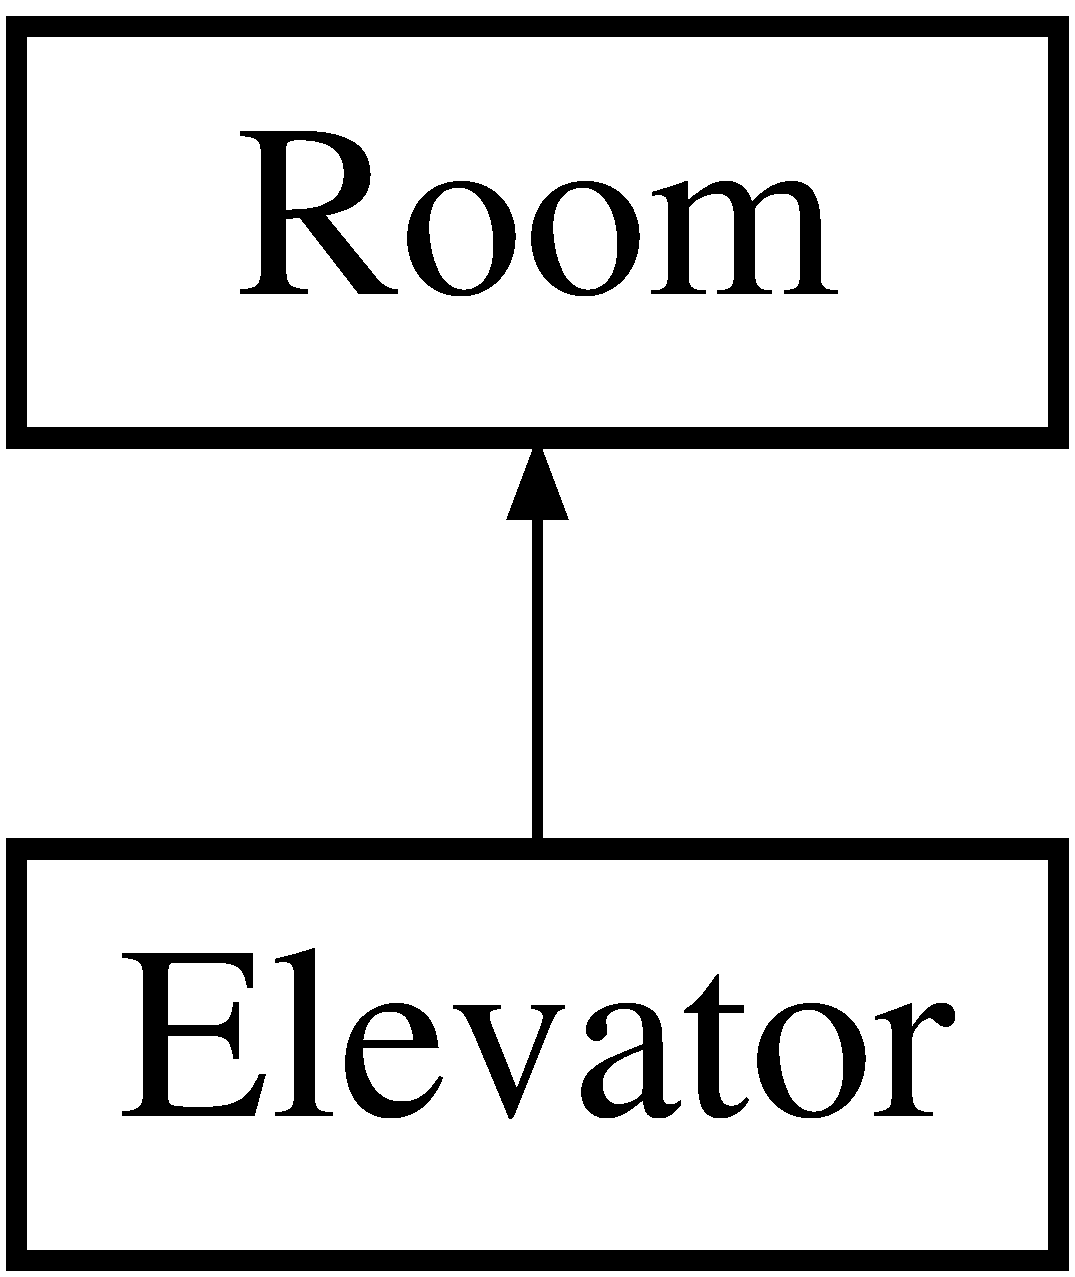
\includegraphics[height=2.000000cm]{classElevator}
\end{center}
\end{figure}
\subsection*{Public Member Functions}
\begin{DoxyCompactItemize}
\item 
\hyperlink{classElevator_af8194f56458803bc090fbd6037f6960c}{Elevator} (String \hyperlink{classRoom_a30e9fb0290f64b567572d2f4b4fac4d9}{name}, String \hyperlink{classRoom_a2f0c64fd0d90618f9c36b935a6f6bb49}{currently}, String \hyperlink{classRoom_ad9e86528519166f3ac3b1413da4e0a41}{heading})
\item 
void \hyperlink{classElevator_a394a3717661c03de38f4c94731b69651}{connect} (\hyperlink{classElevator}{Elevator} down, \hyperlink{classRoom}{Room} connecting\+Room, \hyperlink{classElevator}{Elevator} up)
\item 
String \hyperlink{classElevator_a9af8b09a3eea97a57ac227214aa935ee}{to\+String} ()
\end{DoxyCompactItemize}
\subsection*{Additional Inherited Members}


\subsection{Detailed Description}
Handles the \hyperlink{classElevator}{Elevator}. 

Manages the connections between floors. 

\subsection{Constructor \& Destructor Documentation}
\hypertarget{classElevator_af8194f56458803bc090fbd6037f6960c}{}\index{Elevator@{Elevator}!Elevator@{Elevator}}
\index{Elevator@{Elevator}!Elevator@{Elevator}}
\subsubsection[{Elevator(\+String name, String currently, String heading)}]{\setlength{\rightskip}{0pt plus 5cm}Elevator.\+Elevator (
\begin{DoxyParamCaption}
\item[{String}]{name, }
\item[{String}]{currently, }
\item[{String}]{heading}
\end{DoxyParamCaption}
)\hspace{0.3cm}{\ttfamily [inline]}}\label{classElevator_af8194f56458803bc090fbd6037f6960c}
Creates a new elevator. 
\begin{DoxyParams}{Parameters}
{\em String} & the name of the elevator. \\
\hline
\end{DoxyParams}


\subsection{Member Function Documentation}
\hypertarget{classElevator_a394a3717661c03de38f4c94731b69651}{}\index{Elevator@{Elevator}!connect@{connect}}
\index{connect@{connect}!Elevator@{Elevator}}
\subsubsection[{connect(\+Elevator down, Room connecting\+Room, Elevator up)}]{\setlength{\rightskip}{0pt plus 5cm}void Elevator.\+connect (
\begin{DoxyParamCaption}
\item[{{\bf Elevator}}]{down, }
\item[{{\bf Room}}]{connecting\+Room, }
\item[{{\bf Elevator}}]{up}
\end{DoxyParamCaption}
)\hspace{0.3cm}{\ttfamily [inline]}}\label{classElevator_a394a3717661c03de38f4c94731b69651}
Connects the rooms together 
\begin{DoxyParams}{Parameters}
{\em \hyperlink{classRoom}{Room}} & new floor \\
\hline
\end{DoxyParams}
\hypertarget{classElevator_a9af8b09a3eea97a57ac227214aa935ee}{}\index{Elevator@{Elevator}!to\+String@{to\+String}}
\index{to\+String@{to\+String}!Elevator@{Elevator}}
\subsubsection[{to\+String()}]{\setlength{\rightskip}{0pt plus 5cm}String Elevator.\+to\+String (
\begin{DoxyParamCaption}
{}
\end{DoxyParamCaption}
)\hspace{0.3cm}{\ttfamily [inline]}}\label{classElevator_a9af8b09a3eea97a57ac227214aa935ee}
Converts the \hyperlink{classElevator}{Elevator} to String representation \begin{DoxyReturn}{Returns}
String representation of \hyperlink{classElevator}{Elevator} class 
\end{DoxyReturn}


The documentation for this class was generated from the following file\+:\begin{DoxyCompactItemize}
\item 
Elevator.\+java\end{DoxyCompactItemize}

\hypertarget{classGame}{}\section{Game Class Reference}
\label{classGame}\index{Game@{Game}}


The Game-\/class is responisible for the runtime of the game, taking player inputs and updating the world.  


\subsection*{Static Public Member Functions}
\begin{DoxyCompactItemize}
\item 
static void \hyperlink{classGame_a612ca57db4b230ac5d927e72519ea571}{S\+E\+P\+A\+R\+A\+T\+O\+R} (int i)
\item 
static void \hyperlink{classGame_a98681c889936305d2ffbc2c368e73c88}{create\+Player} ()
\item 
static void \hyperlink{classGame_abb39f1316ab523fbcda8a5ba115927f6}{get\+Help} ()
\item 
static void \hyperlink{classGame_a53324252827f9f298f67ee4c46675029}{quit\+Action} ()
\item 
static void \hyperlink{classGame_a082940112ca18cad8c195c1da0bf4af3}{game\+Status} ()
\item 
static void \hyperlink{classGame_a730e4053e3dbc100c3bc54bb18d20afd}{move\+Action} (int direction)
\begin{DoxyCompactList}\small\item\em Handles movement of the player. \end{DoxyCompactList}\item 
static void \hyperlink{classGame_abe6ec2322cdfa5005ccccd8b07d789fe}{unlock\+Action} (int direction)
\begin{DoxyCompactList}\small\item\em Handles the unlocking of doors. \end{DoxyCompactList}\item 
static void \hyperlink{classGame_a471f2605a676fc54b9b7b6f2d1b628bf}{drop\+Action} (int index)
\begin{DoxyCompactList}\small\item\em handles the dropping of items from player inventory \end{DoxyCompactList}\item 
\hypertarget{classGame_afd5edfadde47ff28830341b56a7112c1}{}static void \hyperlink{classGame_afd5edfadde47ff28830341b56a7112c1}{people\+Action} ()\label{classGame_afd5edfadde47ff28830341b56a7112c1}

\begin{DoxyCompactList}\small\item\em Handles interactions with people in the \hyperlink{classRoom}{Room}. \end{DoxyCompactList}\item 
\hypertarget{classGame_ae52595a27ac1b327b05db2129ad81fca}{}static void {\bfseries main} (String\mbox{[}$\,$\mbox{]} args)\label{classGame_ae52595a27ac1b327b05db2129ad81fca}

\end{DoxyCompactItemize}


\subsection{Detailed Description}
The Game-\/class is responisible for the runtime of the game, taking player inputs and updating the world. 

This class will handle the inputs and the continues updates to the world during runtime. When it exits the game exits. 

\subsection{Member Function Documentation}
\hypertarget{classGame_a98681c889936305d2ffbc2c368e73c88}{}\index{Game@{Game}!create\+Player@{create\+Player}}
\index{create\+Player@{create\+Player}!Game@{Game}}
\subsubsection[{create\+Player()}]{\setlength{\rightskip}{0pt plus 5cm}static void Game.\+create\+Player (
\begin{DoxyParamCaption}
{}
\end{DoxyParamCaption}
)\hspace{0.3cm}{\ttfamily [inline]}, {\ttfamily [static]}}\label{classGame_a98681c889936305d2ffbc2c368e73c88}
Character creation \hypertarget{classGame_a471f2605a676fc54b9b7b6f2d1b628bf}{}\index{Game@{Game}!drop\+Action@{drop\+Action}}
\index{drop\+Action@{drop\+Action}!Game@{Game}}
\subsubsection[{drop\+Action(int index)}]{\setlength{\rightskip}{0pt plus 5cm}static void Game.\+drop\+Action (
\begin{DoxyParamCaption}
\item[{int}]{index}
\end{DoxyParamCaption}
)\hspace{0.3cm}{\ttfamily [inline]}, {\ttfamily [static]}}\label{classGame_a471f2605a676fc54b9b7b6f2d1b628bf}


handles the dropping of items from player inventory 


\begin{DoxyParams}{Parameters}
{\em int} & Index of the item you wish to drop. \\
\hline
\end{DoxyParams}
\hypertarget{classGame_a082940112ca18cad8c195c1da0bf4af3}{}\index{Game@{Game}!game\+Status@{game\+Status}}
\index{game\+Status@{game\+Status}!Game@{Game}}
\subsubsection[{game\+Status()}]{\setlength{\rightskip}{0pt plus 5cm}static void Game.\+game\+Status (
\begin{DoxyParamCaption}
{}
\end{DoxyParamCaption}
)\hspace{0.3cm}{\ttfamily [inline]}, {\ttfamily [static]}}\label{classGame_a082940112ca18cad8c195c1da0bf4af3}
Prints the status of the game to the std-\/output \hypertarget{classGame_abb39f1316ab523fbcda8a5ba115927f6}{}\index{Game@{Game}!get\+Help@{get\+Help}}
\index{get\+Help@{get\+Help}!Game@{Game}}
\subsubsection[{get\+Help()}]{\setlength{\rightskip}{0pt plus 5cm}static void Game.\+get\+Help (
\begin{DoxyParamCaption}
{}
\end{DoxyParamCaption}
)\hspace{0.3cm}{\ttfamily [inline]}, {\ttfamily [static]}}\label{classGame_abb39f1316ab523fbcda8a5ba115927f6}
Prints the help-\/section of the game to the terminal. \hypertarget{classGame_a730e4053e3dbc100c3bc54bb18d20afd}{}\index{Game@{Game}!move\+Action@{move\+Action}}
\index{move\+Action@{move\+Action}!Game@{Game}}
\subsubsection[{move\+Action(int direction)}]{\setlength{\rightskip}{0pt plus 5cm}static void Game.\+move\+Action (
\begin{DoxyParamCaption}
\item[{int}]{direction}
\end{DoxyParamCaption}
)\hspace{0.3cm}{\ttfamily [inline]}, {\ttfamily [static]}}\label{classGame_a730e4053e3dbc100c3bc54bb18d20afd}


Handles movement of the player. 

The directions are\+:~\newline
 0=North ~\newline
 1=East ~\newline
 2=West ~\newline
 3=South ~\newline
 4=Down ~\newline
 5=Up ~\newline

\begin{DoxyParams}{Parameters}
{\em int} & representing a direction () \\
\hline
\end{DoxyParams}
\hypertarget{classGame_a53324252827f9f298f67ee4c46675029}{}\index{Game@{Game}!quit\+Action@{quit\+Action}}
\index{quit\+Action@{quit\+Action}!Game@{Game}}
\subsubsection[{quit\+Action()}]{\setlength{\rightskip}{0pt plus 5cm}static void Game.\+quit\+Action (
\begin{DoxyParamCaption}
{}
\end{DoxyParamCaption}
)\hspace{0.3cm}{\ttfamily [inline]}, {\ttfamily [static]}}\label{classGame_a53324252827f9f298f67ee4c46675029}
Promts the player if he/she really wants to quit the game. \hypertarget{classGame_a612ca57db4b230ac5d927e72519ea571}{}\index{Game@{Game}!S\+E\+P\+A\+R\+A\+T\+O\+R@{S\+E\+P\+A\+R\+A\+T\+O\+R}}
\index{S\+E\+P\+A\+R\+A\+T\+O\+R@{S\+E\+P\+A\+R\+A\+T\+O\+R}!Game@{Game}}
\subsubsection[{S\+E\+P\+A\+R\+A\+T\+O\+R(int i)}]{\setlength{\rightskip}{0pt plus 5cm}static void Game.\+S\+E\+P\+A\+R\+A\+T\+O\+R (
\begin{DoxyParamCaption}
\item[{int}]{i}
\end{DoxyParamCaption}
)\hspace{0.3cm}{\ttfamily [inline]}, {\ttfamily [static]}}\label{classGame_a612ca57db4b230ac5d927e72519ea571}
Used to print out a series of \char`\"{}\#\char`\"{} to separate lines. 
\begin{DoxyParams}{Parameters}
{\em int} & amount of \#s. \\
\hline
\end{DoxyParams}
\hypertarget{classGame_abe6ec2322cdfa5005ccccd8b07d789fe}{}\index{Game@{Game}!unlock\+Action@{unlock\+Action}}
\index{unlock\+Action@{unlock\+Action}!Game@{Game}}
\subsubsection[{unlock\+Action(int direction)}]{\setlength{\rightskip}{0pt plus 5cm}static void Game.\+unlock\+Action (
\begin{DoxyParamCaption}
\item[{int}]{direction}
\end{DoxyParamCaption}
)\hspace{0.3cm}{\ttfamily [inline]}, {\ttfamily [static]}}\label{classGame_abe6ec2322cdfa5005ccccd8b07d789fe}


Handles the unlocking of doors. 

The directions are\+: 0=North ~\newline
 1=East ~\newline
 2=West ~\newline
 3=South ~\newline

\begin{DoxyParams}{Parameters}
{\em int} & The direction \\
\hline
\end{DoxyParams}


The documentation for this class was generated from the following file\+:\begin{DoxyCompactItemize}
\item 
Game.\+java\end{DoxyCompactItemize}

\hypertarget{classInventory}{}\section{Inventory Class Reference}
\label{classInventory}\index{Inventory@{Inventory}}


Class resposible for different inventorys such as the avatars backpack.  


\subsection*{Public Member Functions}
\begin{DoxyCompactItemize}
\item 
\hyperlink{classInventory_a0c1b37cfe68e9826b61ceadd9e360744}{Inventory} (int max\+Capacity)
\begin{DoxyCompactList}\small\item\em Handles the creation of a new \hyperlink{classInventory}{Inventory}. \end{DoxyCompactList}\item 
boolean \hyperlink{classInventory_ae88a0b1d1058d925daa87a5a8c514d55}{add\+Key} ()
\item 
boolean \hyperlink{classInventory_a2f51b9650e3b6b72c790ce70af2807b4}{contain\+Key} ()
\item 
boolean \hyperlink{classInventory_a650574968bd49dd7f530d9be365b1eac}{remove\+Key} ()
\item 
boolean \hyperlink{classInventory_a9b72524737dae6d453a5a3e34732c8d8}{add\+Book} (\hyperlink{classBook}{Book} new\+Book)
\begin{DoxyCompactList}\small\item\em Adds a book to the inventory. \end{DoxyCompactList}\item 
\hyperlink{classBook}{Book} \hyperlink{classInventory_a2401c8b134a26ce2f50b70a0d913a5af}{get\+Book} (int index)
\begin{DoxyCompactList}\small\item\em Gets the book at index. \end{DoxyCompactList}\item 
boolean \hyperlink{classInventory_a79e7dfaa4acec1562a8eca51f4935146}{remove\+Book} (int index)
\begin{DoxyCompactList}\small\item\em Removes the book at provided index. \end{DoxyCompactList}\item 
int \hyperlink{classInventory_ac663a5a8da5d711b8bc158193114f0e6}{books\+Quantity} ()
\begin{DoxyCompactList}\small\item\em Fetches how many books are currently in the inventory. \end{DoxyCompactList}\item 
void \hyperlink{classInventory_a6965b4166b280d887b8c54c6c46b099b}{print} ()
\end{DoxyCompactItemize}


\subsection{Detailed Description}
Class resposible for different inventorys such as the avatars backpack. 

\subsection{Constructor \& Destructor Documentation}
\hypertarget{classInventory_a0c1b37cfe68e9826b61ceadd9e360744}{}\index{Inventory@{Inventory}!Inventory@{Inventory}}
\index{Inventory@{Inventory}!Inventory@{Inventory}}
\subsubsection[{Inventory(int max\+Capacity)}]{\setlength{\rightskip}{0pt plus 5cm}Inventory.\+Inventory (
\begin{DoxyParamCaption}
\item[{int}]{max\+Capacity}
\end{DoxyParamCaption}
)\hspace{0.3cm}{\ttfamily [inline]}}\label{classInventory_a0c1b37cfe68e9826b61ceadd9e360744}


Handles the creation of a new \hyperlink{classInventory}{Inventory}. 


\begin{DoxyParams}{Parameters}
{\em int} & max\+Capacity \\
\hline
\end{DoxyParams}


\subsection{Member Function Documentation}
\hypertarget{classInventory_a9b72524737dae6d453a5a3e34732c8d8}{}\index{Inventory@{Inventory}!add\+Book@{add\+Book}}
\index{add\+Book@{add\+Book}!Inventory@{Inventory}}
\subsubsection[{add\+Book(\+Book new\+Book)}]{\setlength{\rightskip}{0pt plus 5cm}boolean Inventory.\+add\+Book (
\begin{DoxyParamCaption}
\item[{{\bf Book}}]{new\+Book}
\end{DoxyParamCaption}
)\hspace{0.3cm}{\ttfamily [inline]}}\label{classInventory_a9b72524737dae6d453a5a3e34732c8d8}


Adds a book to the inventory. 


\begin{DoxyParams}{Parameters}
{\em \hyperlink{classBook}{Book}} & true if successfull, false if not \\
\hline
\end{DoxyParams}
\hypertarget{classInventory_ae88a0b1d1058d925daa87a5a8c514d55}{}\index{Inventory@{Inventory}!add\+Key@{add\+Key}}
\index{add\+Key@{add\+Key}!Inventory@{Inventory}}
\subsubsection[{add\+Key()}]{\setlength{\rightskip}{0pt plus 5cm}boolean Inventory.\+add\+Key (
\begin{DoxyParamCaption}
{}
\end{DoxyParamCaption}
)\hspace{0.3cm}{\ttfamily [inline]}}\label{classInventory_ae88a0b1d1058d925daa87a5a8c514d55}
Adds a key to the player \hyperlink{classInventory}{Inventory} \begin{DoxyReturn}{Returns}
true if Successfull add, false if \hyperlink{classInventory}{Inventory} is full. 
\end{DoxyReturn}
\hypertarget{classInventory_ac663a5a8da5d711b8bc158193114f0e6}{}\index{Inventory@{Inventory}!books\+Quantity@{books\+Quantity}}
\index{books\+Quantity@{books\+Quantity}!Inventory@{Inventory}}
\subsubsection[{books\+Quantity()}]{\setlength{\rightskip}{0pt plus 5cm}int Inventory.\+books\+Quantity (
\begin{DoxyParamCaption}
{}
\end{DoxyParamCaption}
)\hspace{0.3cm}{\ttfamily [inline]}}\label{classInventory_ac663a5a8da5d711b8bc158193114f0e6}


Fetches how many books are currently in the inventory. 

\begin{DoxyReturn}{Returns}
int Amount of books in inventory 
\end{DoxyReturn}
\hypertarget{classInventory_a2f51b9650e3b6b72c790ce70af2807b4}{}\index{Inventory@{Inventory}!contain\+Key@{contain\+Key}}
\index{contain\+Key@{contain\+Key}!Inventory@{Inventory}}
\subsubsection[{contain\+Key()}]{\setlength{\rightskip}{0pt plus 5cm}boolean Inventory.\+contain\+Key (
\begin{DoxyParamCaption}
{}
\end{DoxyParamCaption}
)\hspace{0.3cm}{\ttfamily [inline]}}\label{classInventory_a2f51b9650e3b6b72c790ce70af2807b4}
Checks if there is any keys in the inventory \begin{DoxyReturn}{Returns}
boolean true if there are, false if not. 
\end{DoxyReturn}
\hypertarget{classInventory_a2401c8b134a26ce2f50b70a0d913a5af}{}\index{Inventory@{Inventory}!get\+Book@{get\+Book}}
\index{get\+Book@{get\+Book}!Inventory@{Inventory}}
\subsubsection[{get\+Book(int index)}]{\setlength{\rightskip}{0pt plus 5cm}{\bf Book} Inventory.\+get\+Book (
\begin{DoxyParamCaption}
\item[{int}]{index}
\end{DoxyParamCaption}
)\hspace{0.3cm}{\ttfamily [inline]}}\label{classInventory_a2401c8b134a26ce2f50b70a0d913a5af}


Gets the book at index. 


\begin{DoxyParams}{Parameters}
{\em int} & index of the book \\
\hline
\end{DoxyParams}
\begin{DoxyReturn}{Returns}
\hyperlink{classBook}{Book} if index is in range, otherwise null 
\end{DoxyReturn}
\hypertarget{classInventory_a6965b4166b280d887b8c54c6c46b099b}{}\index{Inventory@{Inventory}!print@{print}}
\index{print@{print}!Inventory@{Inventory}}
\subsubsection[{print()}]{\setlength{\rightskip}{0pt plus 5cm}void Inventory.\+print (
\begin{DoxyParamCaption}
{}
\end{DoxyParamCaption}
)\hspace{0.3cm}{\ttfamily [inline]}}\label{classInventory_a6965b4166b280d887b8c54c6c46b099b}
Prints the \hyperlink{classInventory}{Inventory} to std-\/output \hypertarget{classInventory_a79e7dfaa4acec1562a8eca51f4935146}{}\index{Inventory@{Inventory}!remove\+Book@{remove\+Book}}
\index{remove\+Book@{remove\+Book}!Inventory@{Inventory}}
\subsubsection[{remove\+Book(int index)}]{\setlength{\rightskip}{0pt plus 5cm}boolean Inventory.\+remove\+Book (
\begin{DoxyParamCaption}
\item[{int}]{index}
\end{DoxyParamCaption}
)\hspace{0.3cm}{\ttfamily [inline]}}\label{classInventory_a79e7dfaa4acec1562a8eca51f4935146}


Removes the book at provided index. 


\begin{DoxyParams}{Parameters}
{\em int} & Index of the book to removes \\
\hline
\end{DoxyParams}
\begin{DoxyReturn}{Returns}
boolean true if successfull, false if not 
\end{DoxyReturn}
\hypertarget{classInventory_a650574968bd49dd7f530d9be365b1eac}{}\index{Inventory@{Inventory}!remove\+Key@{remove\+Key}}
\index{remove\+Key@{remove\+Key}!Inventory@{Inventory}}
\subsubsection[{remove\+Key()}]{\setlength{\rightskip}{0pt plus 5cm}boolean Inventory.\+remove\+Key (
\begin{DoxyParamCaption}
{}
\end{DoxyParamCaption}
)\hspace{0.3cm}{\ttfamily [inline]}}\label{classInventory_a650574968bd49dd7f530d9be365b1eac}
Removes a key from the inventory \begin{DoxyReturn}{Returns}
boolean true if sucessfull, false if not 
\end{DoxyReturn}


The documentation for this class was generated from the following file\+:\begin{DoxyCompactItemize}
\item 
Inventory.\+java\end{DoxyCompactItemize}

\hypertarget{classNPC}{}\section{N\+P\+C Class Reference}
\label{classNPC}\index{N\+P\+C@{N\+P\+C}}


The N\+P\+C-\/class handles the different kinds of N\+P\+Cs in the game.  


Inheritance diagram for N\+P\+C\+:\begin{figure}[H]
\begin{center}
\leavevmode
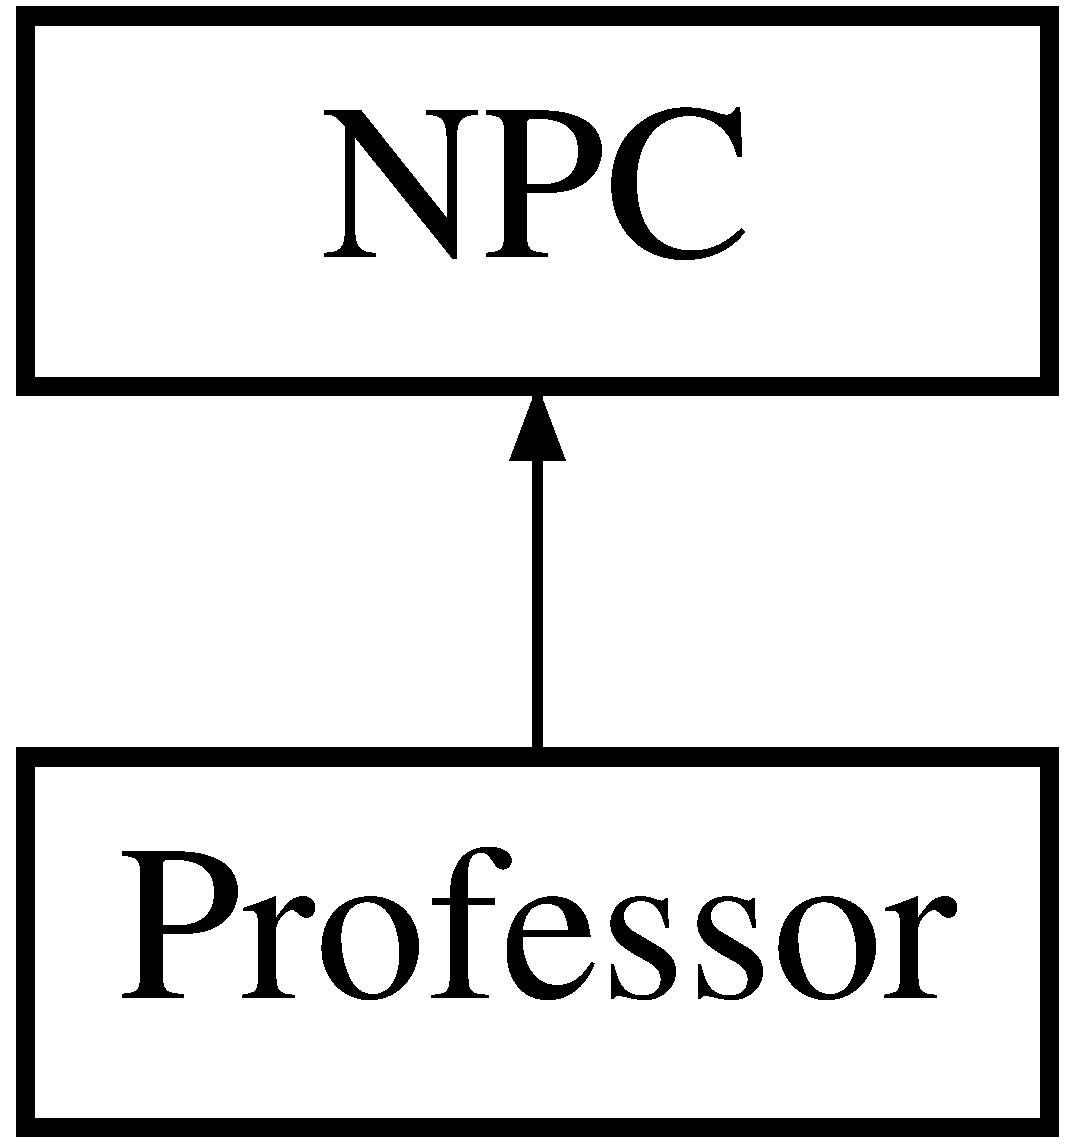
\includegraphics[height=2.000000cm]{classNPC}
\end{center}
\end{figure}
\subsection*{Public Member Functions}
\begin{DoxyCompactItemize}
\item 
\hyperlink{classNPC_aeda507dafafcbe227ef1b9fddb16a81c}{N\+P\+C} (String \hyperlink{classNPC_aea85d6c8ba3ff811f54571fde45f5329}{name})
\item 
String \hyperlink{classNPC_af92732b6477b26c4c8b08cf6b18b116f}{get\+Name} ()
\end{DoxyCompactItemize}
\subsection*{Protected Attributes}
\begin{DoxyCompactItemize}
\item 
String \hyperlink{classNPC_aea85d6c8ba3ff811f54571fde45f5329}{name}
\end{DoxyCompactItemize}


\subsection{Detailed Description}
The N\+P\+C-\/class handles the different kinds of N\+P\+Cs in the game. 

The \hyperlink{classNPC}{N\+P\+C} can be either a student or a professor (More might come). Things that they all have includes name, type(\+Student, Prof), action(dialog, question, etc), inventory(\+Keys, test, etc). The best way to use this might be to let two new classes, student and professor, inherit the \hyperlink{classNPC}{N\+P\+C} class. 

\subsection{Constructor \& Destructor Documentation}
\hypertarget{classNPC_aeda507dafafcbe227ef1b9fddb16a81c}{}\index{N\+P\+C@{N\+P\+C}!N\+P\+C@{N\+P\+C}}
\index{N\+P\+C@{N\+P\+C}!N\+P\+C@{N\+P\+C}}
\subsubsection[{N\+P\+C(\+String name)}]{\setlength{\rightskip}{0pt plus 5cm}N\+P\+C.\+N\+P\+C (
\begin{DoxyParamCaption}
\item[{String}]{name}
\end{DoxyParamCaption}
)\hspace{0.3cm}{\ttfamily [inline]}}\label{classNPC_aeda507dafafcbe227ef1b9fddb16a81c}
Creates a new \hyperlink{classNPC}{N\+P\+C} with specified name. 
\begin{DoxyParams}{Parameters}
{\em String} & the name of the \hyperlink{classNPC}{N\+P\+C}. \\
\hline
\end{DoxyParams}


\subsection{Member Function Documentation}
\hypertarget{classNPC_af92732b6477b26c4c8b08cf6b18b116f}{}\index{N\+P\+C@{N\+P\+C}!get\+Name@{get\+Name}}
\index{get\+Name@{get\+Name}!N\+P\+C@{N\+P\+C}}
\subsubsection[{get\+Name()}]{\setlength{\rightskip}{0pt plus 5cm}String N\+P\+C.\+get\+Name (
\begin{DoxyParamCaption}
{}
\end{DoxyParamCaption}
)\hspace{0.3cm}{\ttfamily [inline]}}\label{classNPC_af92732b6477b26c4c8b08cf6b18b116f}
the name of the \hyperlink{classNPC}{N\+P\+C} 

\subsection{Member Data Documentation}
\hypertarget{classNPC_aea85d6c8ba3ff811f54571fde45f5329}{}\index{N\+P\+C@{N\+P\+C}!name@{name}}
\index{name@{name}!N\+P\+C@{N\+P\+C}}
\subsubsection[{name}]{\setlength{\rightskip}{0pt plus 5cm}String N\+P\+C.\+name\hspace{0.3cm}{\ttfamily [protected]}}\label{classNPC_aea85d6c8ba3ff811f54571fde45f5329}
The name of the \hyperlink{classNPC}{N\+P\+C}. 

The documentation for this class was generated from the following file\+:\begin{DoxyCompactItemize}
\item 
N\+P\+C.\+java\end{DoxyCompactItemize}

\hypertarget{classProfessor}{}\section{Professor Class Reference}
\label{classProfessor}\index{Professor@{Professor}}


Sub class of \hyperlink{classNPC}{N\+P\+C}.  


Inheritance diagram for Professor\+:\begin{figure}[H]
\begin{center}
\leavevmode
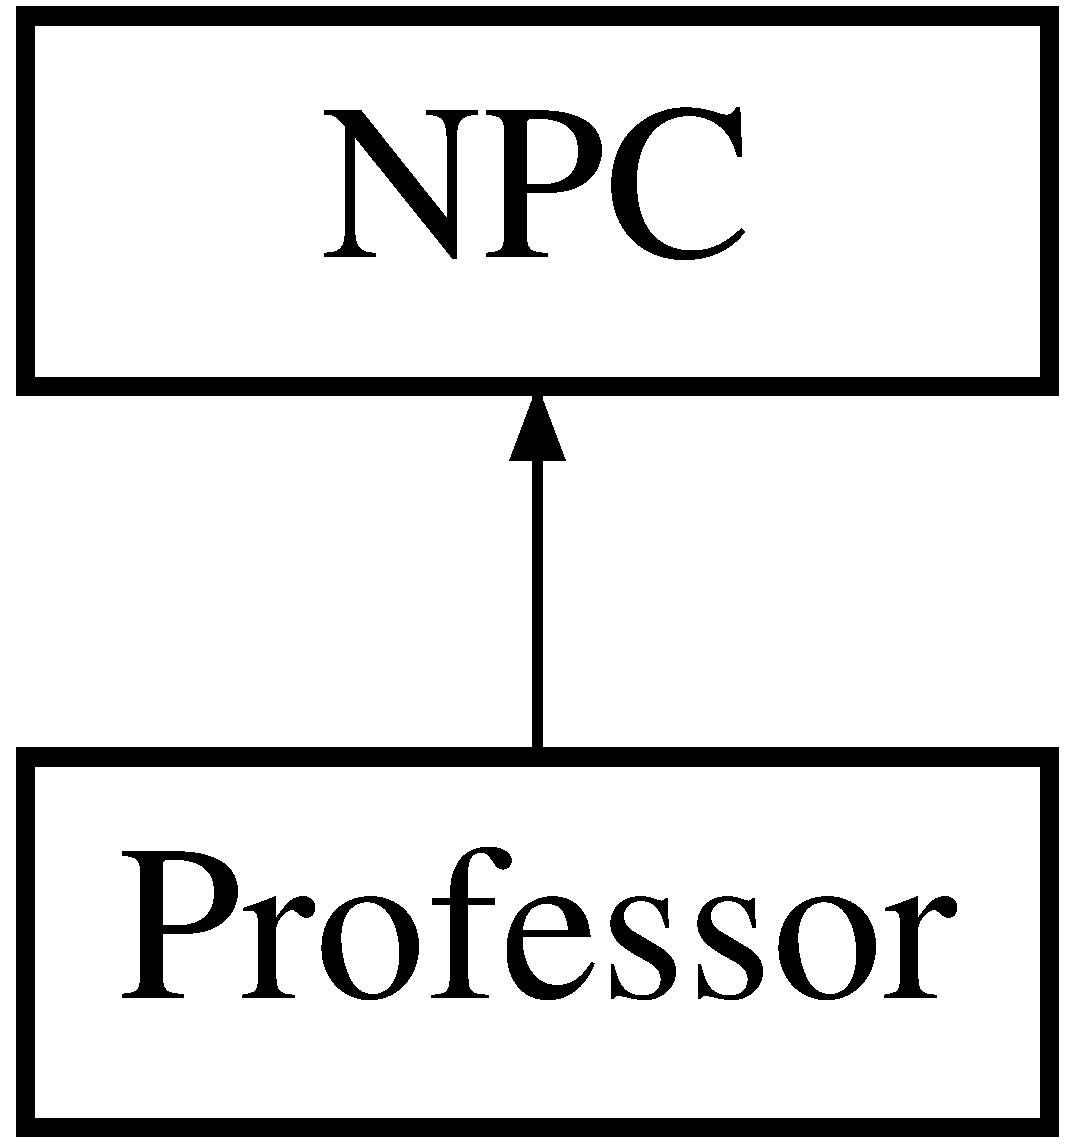
\includegraphics[height=2.000000cm]{classProfessor}
\end{center}
\end{figure}
\subsection*{Public Member Functions}
\begin{DoxyCompactItemize}
\item 
\hypertarget{classProfessor_ad5d9f88c7887d9cc34678643c9e2aa9b}{}{\bfseries Professor} (String \hyperlink{classNPC_aea85d6c8ba3ff811f54571fde45f5329}{name}, int course\+I\+D)\label{classProfessor_ad5d9f88c7887d9cc34678643c9e2aa9b}

\item 
\hypertarget{classProfessor_a116ed1d5348bb5071f75d031ded48147}{}String \hyperlink{classProfessor_a116ed1d5348bb5071f75d031ded48147}{get\+Course} ()\label{classProfessor_a116ed1d5348bb5071f75d031ded48147}

\begin{DoxyCompactList}\small\item\em Fetches the course the professor is bound to. \end{DoxyCompactList}\item 
\hypertarget{classProfessor_ad341254c6e6a4f8f86e54b65d148008b}{}String \hyperlink{classProfessor_ad341254c6e6a4f8f86e54b65d148008b}{to\+String} ()\label{classProfessor_ad341254c6e6a4f8f86e54b65d148008b}

\begin{DoxyCompactList}\small\item\em Makes String representation of a professor. \end{DoxyCompactList}\item 
\hypertarget{classProfessor_ab9d19baf3798b2e827c3f7db3b08845e}{}void \hyperlink{classProfessor_ab9d19baf3798b2e827c3f7db3b08845e}{print} ()\label{classProfessor_ab9d19baf3798b2e827c3f7db3b08845e}

\begin{DoxyCompactList}\small\item\em Prints the professor. \end{DoxyCompactList}\end{DoxyCompactItemize}
\subsection*{Additional Inherited Members}


\subsection{Detailed Description}
Sub class of \hyperlink{classNPC}{N\+P\+C}. 

A \hyperlink{classProfessor}{Professor} is a special type of \hyperlink{classNPC}{N\+P\+C}, which is linked to a course. He/she can ask questions about the course and give the \hyperlink{classAvatar}{Avatar} H\+P. 

The documentation for this class was generated from the following file\+:\begin{DoxyCompactItemize}
\item 
Professor.\+java\end{DoxyCompactItemize}

\hypertarget{classRoom}{}\section{Room Class Reference}
\label{classRoom}\index{Room@{Room}}


The Room-\/class managing all the functions related to the rooms.  


Inheritance diagram for Room\+:\begin{figure}[H]
\begin{center}
\leavevmode
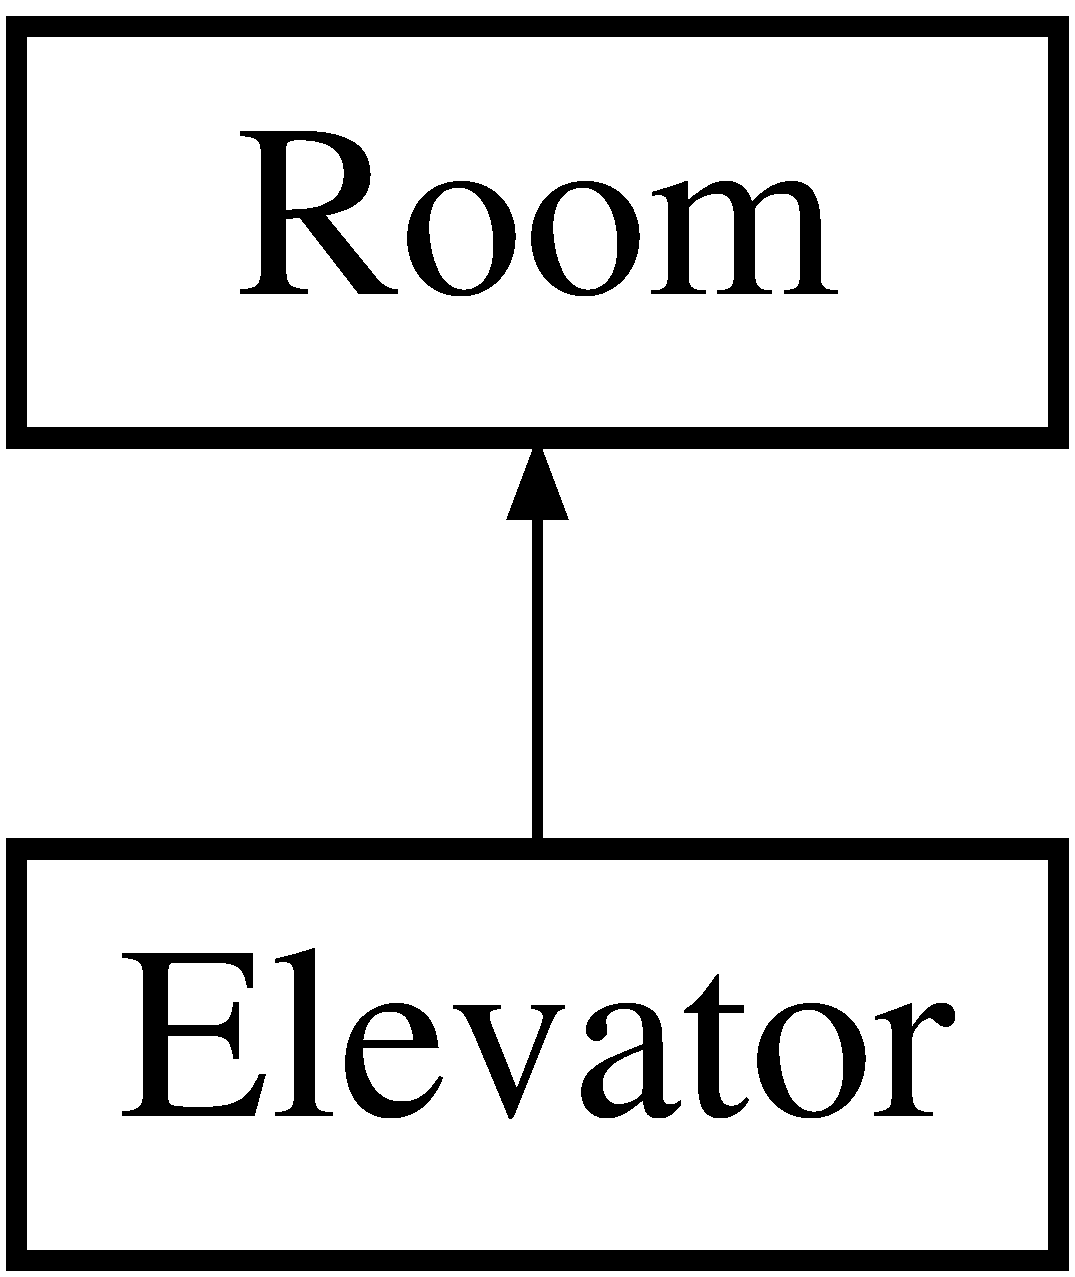
\includegraphics[height=2.000000cm]{classRoom}
\end{center}
\end{figure}
\subsection*{Public Member Functions}
\begin{DoxyCompactItemize}
\item 
\hyperlink{classRoom_ae162f5cbb105a45bb5b72adcccfd250f}{Room} (String \hyperlink{classRoom_a30e9fb0290f64b567572d2f4b4fac4d9}{name}, String \hyperlink{classRoom_a2f0c64fd0d90618f9c36b935a6f6bb49}{currently}, String \hyperlink{classRoom_ad9e86528519166f3ac3b1413da4e0a41}{heading})
\begin{DoxyCompactList}\small\item\em Creates a room. \end{DoxyCompactList}\item 
void \hyperlink{classRoom_af82990e218a9dced9c6226b0083bfb8a}{connect} (\hyperlink{classRoom}{Room} n, \hyperlink{classRoom}{Room} e, \hyperlink{classRoom}{Room} w, \hyperlink{classRoom}{Room} s)
\item 
void \hyperlink{classRoom_a074e41e5dbc41dd4a71cac2a101c1f56}{set\+Locks} (boolean n, boolean e, boolean w, boolean s)
\item 
String \hyperlink{classRoom_aa0c9b6ddd98d29a9cc4e31c6c66a8ea4}{grammer\+Currently} ()
\item 
String \hyperlink{classRoom_a8d2578df19ba7b0d5c76c9567aba83df}{grammer\+Heading} ()
\item 
String \hyperlink{classRoom_ab638bfd4155075a97e6d3ec306b467f0}{get\+Name} ()
\item 
void \hyperlink{classRoom_adefdb50c618b7d7d91fb2025eefc39e0}{set\+Desc} (String desc)
\item 
String \hyperlink{classRoom_ad0996a895179c9ba712e5be94534e58e}{get\+Desc} ()
\item 
void \hyperlink{classRoom_ac6f911c07206b270b6d821f0b9a67a01}{add\+Npc} (\hyperlink{classNPC}{N\+P\+C} npc)
\item 
List$<$ \hyperlink{classNPC}{N\+P\+C} $>$ \hyperlink{classRoom_a0c5b0189a4149e963ac93965acbf8088}{get\+Npc\+List} ()
\item 
String \hyperlink{classRoom_a74ac6cc2152ba812702258b9c4fd70db}{get\+N\+P\+C} (int index)
\begin{DoxyCompactList}\small\item\em Fetches a npc at index. \end{DoxyCompactList}\item 
boolean \hyperlink{classRoom_aff32fa2f3e836c00921e18408a432a0d}{is\+Adjacent\+Unlocked} (int cardinal)
\item 
void \hyperlink{classRoom_ace2ee11dd317462ad17dc457109a30f5}{unlock\+Door} (int cardinal)
\item 
\hyperlink{classRoom}{Room} \hyperlink{classRoom_ae10de76a88deb65efbbcd42d1557da68}{get\+Adjacent\+Room} (int cardinal)
\item 
void \hyperlink{classRoom_ab5fed82dacde130f70941779b0b6c7fb}{add\+Action} (int probability, int action\+I\+D)
\begin{DoxyCompactList}\small\item\em This function adds actions to the room. \end{DoxyCompactList}\item 
void \hyperlink{classRoom_acf497ba6df7779bfbc4786dd069d84ef}{check\+Actions} ()
\item 
void \hyperlink{classRoom_a17dc052da1d8f76adf886352d3523d9f}{run\+Action} (int action\+I\+D)
\begin{DoxyCompactList}\small\item\em This function fetches the right function based on the action\+I\+D. \end{DoxyCompactList}\item 
boolean \hyperlink{classRoom_aef1fd9dd031e99eb01947603bca26918}{is\+An\+Elevator} ()
\item 
boolean \hyperlink{classRoom_a2d753b78a122a29c0a6bf9da4fd2dd6b}{equals} (\hyperlink{classRoom}{Room} comp)
\item 
String \hyperlink{classRoom_a257d76391ce0c9999151358143855a84}{to\+String} ()
\item 
void \hyperlink{classRoom_ad090e030e50a028019930016932789eb}{print} ()
\end{DoxyCompactItemize}
\subsection*{Protected Attributes}
\begin{DoxyCompactItemize}
\item 
String \hyperlink{classRoom_a30e9fb0290f64b567572d2f4b4fac4d9}{name}
\item 
String \hyperlink{classRoom_a2d7ecf802690a6b13750ca6fa6882d77}{description}
\item 
String \hyperlink{classRoom_a2f0c64fd0d90618f9c36b935a6f6bb49}{currently}
\item 
String \hyperlink{classRoom_ad9e86528519166f3ac3b1413da4e0a41}{heading}
\item 
boolean \hyperlink{classRoom_a9ae4a56ee28e7e6cae000555032a8e41}{is\+An\+Elevator} = false
\item 
List$<$ \hyperlink{classRoom}{Room} $>$ \hyperlink{classRoom_a9d060d005fd9719f87f5045656fdf7f0}{adjacent\+Rooms} = new Linked\+List$<$\hyperlink{classRoom}{Room}$>$()
\end{DoxyCompactItemize}


\subsection{Detailed Description}
The Room-\/class managing all the functions related to the rooms. 

Each room will contain different objects and npcs that the Game-\/class can fetch by using functions from this class. 

\subsection{Constructor \& Destructor Documentation}
\hypertarget{classRoom_ae162f5cbb105a45bb5b72adcccfd250f}{}\index{Room@{Room}!Room@{Room}}
\index{Room@{Room}!Room@{Room}}
\subsubsection[{Room(\+String name, String currently, String heading)}]{\setlength{\rightskip}{0pt plus 5cm}Room.\+Room (
\begin{DoxyParamCaption}
\item[{String}]{name, }
\item[{String}]{currently, }
\item[{String}]{heading}
\end{DoxyParamCaption}
)\hspace{0.3cm}{\ttfamily [inline]}}\label{classRoom_ae162f5cbb105a45bb5b72adcccfd250f}


Creates a room. 

Should take rooms in all four cardinals (north, south, etc) as arguments. 
\begin{DoxyParams}{Parameters}
{\em String} & the name of the new room in the form of a String. \\
\hline
{\em String} & the correct words to connect name to \char`\"{}you are currently $<$name$>$\char`\"{} \\
\hline
{\em String} & the correct words to connect name to \char`\"{}you are heading $<$name$>$\char`\"{} \\
\hline
\end{DoxyParams}


\subsection{Member Function Documentation}
\hypertarget{classRoom_ab5fed82dacde130f70941779b0b6c7fb}{}\index{Room@{Room}!add\+Action@{add\+Action}}
\index{add\+Action@{add\+Action}!Room@{Room}}
\subsubsection[{add\+Action(int probability, int action\+I\+D)}]{\setlength{\rightskip}{0pt plus 5cm}void Room.\+add\+Action (
\begin{DoxyParamCaption}
\item[{int}]{probability, }
\item[{int}]{action\+I\+D}
\end{DoxyParamCaption}
)\hspace{0.3cm}{\ttfamily [inline]}}\label{classRoom_ab5fed82dacde130f70941779b0b6c7fb}


This function adds actions to the room. 

action\+I\+Ds\+: ~\newline
 0 -\/ Found key 
\begin{DoxyParams}{Parameters}
{\em int} & probability that the action occurs \\
\hline
{\em int} & action\+I\+D which action it is, see details for all I\+Ds \\
\hline
\end{DoxyParams}
\hypertarget{classRoom_ac6f911c07206b270b6d821f0b9a67a01}{}\index{Room@{Room}!add\+Npc@{add\+Npc}}
\index{add\+Npc@{add\+Npc}!Room@{Room}}
\subsubsection[{add\+Npc(\+N\+P\+C npc)}]{\setlength{\rightskip}{0pt plus 5cm}void Room.\+add\+Npc (
\begin{DoxyParamCaption}
\item[{{\bf N\+P\+C}}]{npc}
\end{DoxyParamCaption}
)\hspace{0.3cm}{\ttfamily [inline]}}\label{classRoom_ac6f911c07206b270b6d821f0b9a67a01}
Adds an \hyperlink{classNPC}{N\+P\+C} to the room. \hypertarget{classRoom_acf497ba6df7779bfbc4786dd069d84ef}{}\index{Room@{Room}!check\+Actions@{check\+Actions}}
\index{check\+Actions@{check\+Actions}!Room@{Room}}
\subsubsection[{check\+Actions()}]{\setlength{\rightskip}{0pt plus 5cm}void Room.\+check\+Actions (
\begin{DoxyParamCaption}
{}
\end{DoxyParamCaption}
)\hspace{0.3cm}{\ttfamily [inline]}}\label{classRoom_acf497ba6df7779bfbc4786dd069d84ef}
This checks and runs the rooms actions \hypertarget{classRoom_af82990e218a9dced9c6226b0083bfb8a}{}\index{Room@{Room}!connect@{connect}}
\index{connect@{connect}!Room@{Room}}
\subsubsection[{connect(\+Room n, Room e, Room w, Room s)}]{\setlength{\rightskip}{0pt plus 5cm}void Room.\+connect (
\begin{DoxyParamCaption}
\item[{{\bf Room}}]{n, }
\item[{{\bf Room}}]{e, }
\item[{{\bf Room}}]{w, }
\item[{{\bf Room}}]{s}
\end{DoxyParamCaption}
)\hspace{0.3cm}{\ttfamily [inline]}}\label{classRoom_af82990e218a9dced9c6226b0083bfb8a}
Connects the room to other rooms. 
\begin{DoxyParams}{Parameters}
{\em \hyperlink{classRoom}{Room}} & n (North) \\
\hline
{\em \hyperlink{classRoom}{Room}} & e (East) \\
\hline
{\em \hyperlink{classRoom}{Room}} & w (West) \\
\hline
{\em \hyperlink{classRoom}{Room}} & s (South) \\
\hline
\end{DoxyParams}
\hypertarget{classRoom_a2d753b78a122a29c0a6bf9da4fd2dd6b}{}\index{Room@{Room}!equals@{equals}}
\index{equals@{equals}!Room@{Room}}
\subsubsection[{equals(\+Room comp)}]{\setlength{\rightskip}{0pt plus 5cm}boolean Room.\+equals (
\begin{DoxyParamCaption}
\item[{{\bf Room}}]{comp}
\end{DoxyParamCaption}
)\hspace{0.3cm}{\ttfamily [inline]}}\label{classRoom_a2d753b78a122a29c0a6bf9da4fd2dd6b}
Function used to compare rooms 
\begin{DoxyParams}{Parameters}
{\em \hyperlink{classRoom}{Room}} & to compare with \\
\hline
\end{DoxyParams}
\hypertarget{classRoom_ae10de76a88deb65efbbcd42d1557da68}{}\index{Room@{Room}!get\+Adjacent\+Room@{get\+Adjacent\+Room}}
\index{get\+Adjacent\+Room@{get\+Adjacent\+Room}!Room@{Room}}
\subsubsection[{get\+Adjacent\+Room(int cardinal)}]{\setlength{\rightskip}{0pt plus 5cm}{\bf Room} Room.\+get\+Adjacent\+Room (
\begin{DoxyParamCaption}
\item[{int}]{cardinal}
\end{DoxyParamCaption}
)\hspace{0.3cm}{\ttfamily [inline]}}\label{classRoom_ae10de76a88deb65efbbcd42d1557da68}
Fetches the connected room at cardinal. 
\begin{DoxyParams}{Parameters}
{\em int} & (0=North, 1=East, 2=West, 3=South) \\
\hline
\end{DoxyParams}
\hypertarget{classRoom_ad0996a895179c9ba712e5be94534e58e}{}\index{Room@{Room}!get\+Desc@{get\+Desc}}
\index{get\+Desc@{get\+Desc}!Room@{Room}}
\subsubsection[{get\+Desc()}]{\setlength{\rightskip}{0pt plus 5cm}String Room.\+get\+Desc (
\begin{DoxyParamCaption}
{}
\end{DoxyParamCaption}
)\hspace{0.3cm}{\ttfamily [inline]}}\label{classRoom_ad0996a895179c9ba712e5be94534e58e}
Gets the description of a room. \begin{DoxyReturn}{Returns}
String description of the room. 
\end{DoxyReturn}
\hypertarget{classRoom_ab638bfd4155075a97e6d3ec306b467f0}{}\index{Room@{Room}!get\+Name@{get\+Name}}
\index{get\+Name@{get\+Name}!Room@{Room}}
\subsubsection[{get\+Name()}]{\setlength{\rightskip}{0pt plus 5cm}String Room.\+get\+Name (
\begin{DoxyParamCaption}
{}
\end{DoxyParamCaption}
)\hspace{0.3cm}{\ttfamily [inline]}}\label{classRoom_ab638bfd4155075a97e6d3ec306b467f0}
Gets the name of a room. \begin{DoxyReturn}{Returns}
String name of the room. 
\end{DoxyReturn}
\hypertarget{classRoom_a74ac6cc2152ba812702258b9c4fd70db}{}\index{Room@{Room}!get\+N\+P\+C@{get\+N\+P\+C}}
\index{get\+N\+P\+C@{get\+N\+P\+C}!Room@{Room}}
\subsubsection[{get\+N\+P\+C(int index)}]{\setlength{\rightskip}{0pt plus 5cm}String Room.\+get\+N\+P\+C (
\begin{DoxyParamCaption}
\item[{int}]{index}
\end{DoxyParamCaption}
)\hspace{0.3cm}{\ttfamily [inline]}}\label{classRoom_a74ac6cc2152ba812702258b9c4fd70db}


Fetches a npc at index. 


\begin{DoxyParams}{Parameters}
{\em int} & Index of the npc \\
\hline
\end{DoxyParams}
\begin{DoxyReturn}{Returns}
String the \hyperlink{classNPC}{N\+P\+C} if it\textquotesingle{}s in range, otherwise null 
\end{DoxyReturn}
\hypertarget{classRoom_a0c5b0189a4149e963ac93965acbf8088}{}\index{Room@{Room}!get\+Npc\+List@{get\+Npc\+List}}
\index{get\+Npc\+List@{get\+Npc\+List}!Room@{Room}}
\subsubsection[{get\+Npc\+List()}]{\setlength{\rightskip}{0pt plus 5cm}List$<${\bf N\+P\+C}$>$ Room.\+get\+Npc\+List (
\begin{DoxyParamCaption}
{}
\end{DoxyParamCaption}
)\hspace{0.3cm}{\ttfamily [inline]}}\label{classRoom_a0c5b0189a4149e963ac93965acbf8088}
Gets a list of the N\+P\+Cs in the room. \hypertarget{classRoom_aa0c9b6ddd98d29a9cc4e31c6c66a8ea4}{}\index{Room@{Room}!grammer\+Currently@{grammer\+Currently}}
\index{grammer\+Currently@{grammer\+Currently}!Room@{Room}}
\subsubsection[{grammer\+Currently()}]{\setlength{\rightskip}{0pt plus 5cm}String Room.\+grammer\+Currently (
\begin{DoxyParamCaption}
{}
\end{DoxyParamCaption}
)\hspace{0.3cm}{\ttfamily [inline]}}\label{classRoom_aa0c9b6ddd98d29a9cc4e31c6c66a8ea4}
Gets the grammer for currently $<$room$>$. \begin{DoxyReturn}{Returns}
String grammer. 
\end{DoxyReturn}
\hypertarget{classRoom_a8d2578df19ba7b0d5c76c9567aba83df}{}\index{Room@{Room}!grammer\+Heading@{grammer\+Heading}}
\index{grammer\+Heading@{grammer\+Heading}!Room@{Room}}
\subsubsection[{grammer\+Heading()}]{\setlength{\rightskip}{0pt plus 5cm}String Room.\+grammer\+Heading (
\begin{DoxyParamCaption}
{}
\end{DoxyParamCaption}
)\hspace{0.3cm}{\ttfamily [inline]}}\label{classRoom_a8d2578df19ba7b0d5c76c9567aba83df}
Gets the grammer for heading $<$room$>$. \begin{DoxyReturn}{Returns}
String grammer. 
\end{DoxyReturn}
\hypertarget{classRoom_aff32fa2f3e836c00921e18408a432a0d}{}\index{Room@{Room}!is\+Adjacent\+Unlocked@{is\+Adjacent\+Unlocked}}
\index{is\+Adjacent\+Unlocked@{is\+Adjacent\+Unlocked}!Room@{Room}}
\subsubsection[{is\+Adjacent\+Unlocked(int cardinal)}]{\setlength{\rightskip}{0pt plus 5cm}boolean Room.\+is\+Adjacent\+Unlocked (
\begin{DoxyParamCaption}
\item[{int}]{cardinal}
\end{DoxyParamCaption}
)\hspace{0.3cm}{\ttfamily [inline]}}\label{classRoom_aff32fa2f3e836c00921e18408a432a0d}
Asks if a certain door is locked. 
\begin{DoxyParams}{Parameters}
{\em int} & (0=North, 1=East, 2=West, 3=South). \\
\hline
\end{DoxyParams}
\begin{DoxyReturn}{Returns}
Boolean true means unlocked, false means locked. 
\end{DoxyReturn}
\hypertarget{classRoom_aef1fd9dd031e99eb01947603bca26918}{}\index{Room@{Room}!is\+An\+Elevator@{is\+An\+Elevator}}
\index{is\+An\+Elevator@{is\+An\+Elevator}!Room@{Room}}
\subsubsection[{is\+An\+Elevator()}]{\setlength{\rightskip}{0pt plus 5cm}boolean Room.\+is\+An\+Elevator (
\begin{DoxyParamCaption}
{}
\end{DoxyParamCaption}
)\hspace{0.3cm}{\ttfamily [inline]}}\label{classRoom_aef1fd9dd031e99eb01947603bca26918}
Function to check if room is an elevator or not \begin{DoxyReturn}{Returns}
boolean true if it is an elevator 
\end{DoxyReturn}
\hypertarget{classRoom_ad090e030e50a028019930016932789eb}{}\index{Room@{Room}!print@{print}}
\index{print@{print}!Room@{Room}}
\subsubsection[{print()}]{\setlength{\rightskip}{0pt plus 5cm}void Room.\+print (
\begin{DoxyParamCaption}
{}
\end{DoxyParamCaption}
)\hspace{0.3cm}{\ttfamily [inline]}}\label{classRoom_ad090e030e50a028019930016932789eb}
Prints the position-\/summary to the terminal. \hypertarget{classRoom_a17dc052da1d8f76adf886352d3523d9f}{}\index{Room@{Room}!run\+Action@{run\+Action}}
\index{run\+Action@{run\+Action}!Room@{Room}}
\subsubsection[{run\+Action(int action\+I\+D)}]{\setlength{\rightskip}{0pt plus 5cm}void Room.\+run\+Action (
\begin{DoxyParamCaption}
\item[{int}]{action\+I\+D}
\end{DoxyParamCaption}
)\hspace{0.3cm}{\ttfamily [inline]}}\label{classRoom_a17dc052da1d8f76adf886352d3523d9f}


This function fetches the right function based on the action\+I\+D. 


\begin{DoxyParams}{Parameters}
{\em int} & action\+I\+D \\
\hline
\end{DoxyParams}
\hypertarget{classRoom_adefdb50c618b7d7d91fb2025eefc39e0}{}\index{Room@{Room}!set\+Desc@{set\+Desc}}
\index{set\+Desc@{set\+Desc}!Room@{Room}}
\subsubsection[{set\+Desc(\+String desc)}]{\setlength{\rightskip}{0pt plus 5cm}void Room.\+set\+Desc (
\begin{DoxyParamCaption}
\item[{String}]{desc}
\end{DoxyParamCaption}
)\hspace{0.3cm}{\ttfamily [inline]}}\label{classRoom_adefdb50c618b7d7d91fb2025eefc39e0}
Gives a description to the room. 
\begin{DoxyParams}{Parameters}
{\em String} & description of the room. \\
\hline
\end{DoxyParams}
\hypertarget{classRoom_a074e41e5dbc41dd4a71cac2a101c1f56}{}\index{Room@{Room}!set\+Locks@{set\+Locks}}
\index{set\+Locks@{set\+Locks}!Room@{Room}}
\subsubsection[{set\+Locks(boolean n, boolean e, boolean w, boolean s)}]{\setlength{\rightskip}{0pt plus 5cm}void Room.\+set\+Locks (
\begin{DoxyParamCaption}
\item[{boolean}]{n, }
\item[{boolean}]{e, }
\item[{boolean}]{w, }
\item[{boolean}]{s}
\end{DoxyParamCaption}
)\hspace{0.3cm}{\ttfamily [inline]}}\label{classRoom_a074e41e5dbc41dd4a71cac2a101c1f56}
Sets the state of the doors in the room to locked or unlocked. \{North, East, West, North\} 
\begin{DoxyParams}{Parameters}
{\em boolean} & n for north door \\
\hline
{\em boolean} & e for east door \\
\hline
{\em boolean} & w for west door \\
\hline
{\em boolean} & s for south door \\
\hline
\end{DoxyParams}
\hypertarget{classRoom_a257d76391ce0c9999151358143855a84}{}\index{Room@{Room}!to\+String@{to\+String}}
\index{to\+String@{to\+String}!Room@{Room}}
\subsubsection[{to\+String()}]{\setlength{\rightskip}{0pt plus 5cm}String Room.\+to\+String (
\begin{DoxyParamCaption}
{}
\end{DoxyParamCaption}
)\hspace{0.3cm}{\ttfamily [inline]}}\label{classRoom_a257d76391ce0c9999151358143855a84}
Makes a string of a room. \begin{DoxyReturn}{Returns}
String representation of a room. 
\end{DoxyReturn}
\hypertarget{classRoom_ace2ee11dd317462ad17dc457109a30f5}{}\index{Room@{Room}!unlock\+Door@{unlock\+Door}}
\index{unlock\+Door@{unlock\+Door}!Room@{Room}}
\subsubsection[{unlock\+Door(int cardinal)}]{\setlength{\rightskip}{0pt plus 5cm}void Room.\+unlock\+Door (
\begin{DoxyParamCaption}
\item[{int}]{cardinal}
\end{DoxyParamCaption}
)\hspace{0.3cm}{\ttfamily [inline]}}\label{classRoom_ace2ee11dd317462ad17dc457109a30f5}
Unlocks the door at cardinal. 
\begin{DoxyParams}{Parameters}
{\em int} & (0=North, 1=East, 2=West, 3=South) \\
\hline
\end{DoxyParams}


\subsection{Member Data Documentation}
\hypertarget{classRoom_a9d060d005fd9719f87f5045656fdf7f0}{}\index{Room@{Room}!adjacent\+Rooms@{adjacent\+Rooms}}
\index{adjacent\+Rooms@{adjacent\+Rooms}!Room@{Room}}
\subsubsection[{adjacent\+Rooms}]{\setlength{\rightskip}{0pt plus 5cm}List$<${\bf Room}$>$ Room.\+adjacent\+Rooms = new Linked\+List$<${\bf Room}$>$()\hspace{0.3cm}{\ttfamily [protected]}}\label{classRoom_a9d060d005fd9719f87f5045656fdf7f0}
The adjacent rooms (0=north, 1=east, 2=west, 3=south). \hypertarget{classRoom_a2f0c64fd0d90618f9c36b935a6f6bb49}{}\index{Room@{Room}!currently@{currently}}
\index{currently@{currently}!Room@{Room}}
\subsubsection[{currently}]{\setlength{\rightskip}{0pt plus 5cm}String Room.\+currently\hspace{0.3cm}{\ttfamily [protected]}}\label{classRoom_a2f0c64fd0d90618f9c36b935a6f6bb49}
Grammer for using it in sentances. \hypertarget{classRoom_a2d7ecf802690a6b13750ca6fa6882d77}{}\index{Room@{Room}!description@{description}}
\index{description@{description}!Room@{Room}}
\subsubsection[{description}]{\setlength{\rightskip}{0pt plus 5cm}String Room.\+description\hspace{0.3cm}{\ttfamily [protected]}}\label{classRoom_a2d7ecf802690a6b13750ca6fa6882d77}
A short description of the room. \hypertarget{classRoom_ad9e86528519166f3ac3b1413da4e0a41}{}\index{Room@{Room}!heading@{heading}}
\index{heading@{heading}!Room@{Room}}
\subsubsection[{heading}]{\setlength{\rightskip}{0pt plus 5cm}String Room.\+heading\hspace{0.3cm}{\ttfamily [protected]}}\label{classRoom_ad9e86528519166f3ac3b1413da4e0a41}
Grammer for using it in sentances. \hypertarget{classRoom_a9ae4a56ee28e7e6cae000555032a8e41}{}\index{Room@{Room}!is\+An\+Elevator@{is\+An\+Elevator}}
\index{is\+An\+Elevator@{is\+An\+Elevator}!Room@{Room}}
\subsubsection[{is\+An\+Elevator}]{\setlength{\rightskip}{0pt plus 5cm}boolean Room.\+is\+An\+Elevator = false\hspace{0.3cm}{\ttfamily [protected]}}\label{classRoom_a9ae4a56ee28e7e6cae000555032a8e41}
Determines if the room is an elevator or not \hypertarget{classRoom_a30e9fb0290f64b567572d2f4b4fac4d9}{}\index{Room@{Room}!name@{name}}
\index{name@{name}!Room@{Room}}
\subsubsection[{name}]{\setlength{\rightskip}{0pt plus 5cm}String Room.\+name\hspace{0.3cm}{\ttfamily [protected]}}\label{classRoom_a30e9fb0290f64b567572d2f4b4fac4d9}
The name of the room. 

The documentation for this class was generated from the following file\+:\begin{DoxyCompactItemize}
\item 
Room.\+java\end{DoxyCompactItemize}

\hypertarget{classTXTReader}{}\section{T\+X\+T\+Reader Class Reference}
\label{classTXTReader}\index{T\+X\+T\+Reader@{T\+X\+T\+Reader}}


The class responisible for handling course info found in txt files.  


\subsection*{Static Public Member Functions}
\begin{DoxyCompactItemize}
\item 
static int \hyperlink{classTXTReader_a0192ce4884c215947120fabf9e4f7d97}{get\+Lines\+File} (String txt\+File)
\begin{DoxyCompactList}\small\item\em Gets how many books the course has. \end{DoxyCompactList}\item 
static int \hyperlink{classTXTReader_a5b841b6280e72959bded19fa507e2385}{get\+Courses\+Amount} ()
\begin{DoxyCompactList}\small\item\em Gets the amount of courses. \end{DoxyCompactList}\item 
\hypertarget{classTXTReader_ae4c57bb2c5f7eb7569bf41b0989d4a8d}{}static \hyperlink{classCourse}{Course} \hyperlink{classTXTReader_ae4c57bb2c5f7eb7569bf41b0989d4a8d}{create\+Random\+Course} ()\label{classTXTReader_ae4c57bb2c5f7eb7569bf41b0989d4a8d}

\begin{DoxyCompactList}\small\item\em Creates a random course  a new random course. \end{DoxyCompactList}\item 
static int \hyperlink{classTXTReader_aa50e32bac584af6a1cd909c15261d313}{get\+Course\+Book\+Amount} (int course\+I\+D)
\begin{DoxyCompactList}\small\item\em Gets how many books the course has. \end{DoxyCompactList}\item 
static String \hyperlink{classTXTReader_a11d27a0cb164ad919af7ce311e891979}{get\+Course\+Name} (int course\+I\+D)
\begin{DoxyCompactList}\small\item\em Fetches the name of the course bound to the provided id. \end{DoxyCompactList}\item 
static String \hyperlink{classTXTReader_ac3d0b99bc3ead4160cc94d3a418b3097}{get\+Course\+H\+P} (int course\+I\+D)
\begin{DoxyCompactList}\small\item\em Gets the courses H\+P value. \end{DoxyCompactList}\item 
static String \hyperlink{classTXTReader_aa0408f4283bdcb82f45a2147fb38faac}{get\+Course\+Book\+File} (int course\+I\+D)
\begin{DoxyCompactList}\small\item\em Fetches the name of the \hyperlink{classBook}{Book} txt-\/file for the course. \end{DoxyCompactList}\item 
static String \hyperlink{classTXTReader_a420d2835e023f7f0d854a7b64abe6995}{get\+Prof\+Name\+File} (int course\+I\+D)
\begin{DoxyCompactList}\small\item\em Fetches the name of the \hyperlink{classProfessor}{Professor} txt-\/\+File for the course. \end{DoxyCompactList}\item 
\hypertarget{classTXTReader_a75d2e79aa94ebe63749d7806dcf9aa60}{}static void \hyperlink{classTXTReader_a75d2e79aa94ebe63749d7806dcf9aa60}{print\+Course} (int course\+I\+D)\label{classTXTReader_a75d2e79aa94ebe63749d7806dcf9aa60}

\begin{DoxyCompactList}\small\item\em Prints the course. \end{DoxyCompactList}\item 
static int \hyperlink{classTXTReader_a0259986abc13a647e9993a81b411c88e}{random\+Num} (int min, int max)
\begin{DoxyCompactList}\small\item\em Random generator for action-\/probability. \end{DoxyCompactList}\item 
\hypertarget{classTXTReader_ad93e1af501d95cc21916efee0a641968}{}static \hyperlink{classProfessor}{Professor} \hyperlink{classTXTReader_ad93e1af501d95cc21916efee0a641968}{create\+Random\+Prof} ()\label{classTXTReader_ad93e1af501d95cc21916efee0a641968}

\begin{DoxyCompactList}\small\item\em Created a professor with a random name. \end{DoxyCompactList}\item 
static int \hyperlink{classTXTReader_a18295e9e805a64f52a8b164f0698d2a5}{get\+Course\+Prof\+Amount} (int course\+I\+D)
\begin{DoxyCompactList}\small\item\em Gets the amount of lines in the \hyperlink{classProfessor}{Professor} txt-\/file. \end{DoxyCompactList}\item 
static String \hyperlink{classTXTReader_a2d77be92793ade8320fddd1c2cd978fe}{get\+Prof\+Name} (int course\+I\+D, int name\+I\+D)
\begin{DoxyCompactList}\small\item\em Fetches a name from the \hyperlink{classProfessor}{Professor} txt-\/file. \end{DoxyCompactList}\item 
\hypertarget{classTXTReader_ab9a5af64c8939de376aa520d10c55d9a}{}static \hyperlink{classBook}{Book} \hyperlink{classTXTReader_ab9a5af64c8939de376aa520d10c55d9a}{create\+Random\+Book} ()\label{classTXTReader_ab9a5af64c8939de376aa520d10c55d9a}

\begin{DoxyCompactList}\small\item\em Creates a random book from a random course. \end{DoxyCompactList}\item 
static String \hyperlink{classTXTReader_a59c8c95a6436b27076bc57c123db3c63}{get\+Book\+Name} (int course\+I\+D, int book\+I\+D)
\begin{DoxyCompactList}\small\item\em Gets the name of the book specified by the provided index. \end{DoxyCompactList}\item 
static String \hyperlink{classTXTReader_a595b7f527438b44072b25de0410170fd}{get\+Book\+Author} (int course\+I\+D, int book\+I\+D)
\begin{DoxyCompactList}\small\item\em Gets the name of the author to the book specified by the provided index. \end{DoxyCompactList}\item 
static int \hyperlink{classTXTReader_aaca34258d8e4a8370e5bb58b497bb8bc}{get\+Book\+Year} (int course\+I\+D, int book\+I\+D)
\begin{DoxyCompactList}\small\item\em Gets the year when the book was published. \end{DoxyCompactList}\item 
static int \hyperlink{classTXTReader_a5c3b8e4474da76fcf6cfe46434c71d29}{get\+Book\+Size} (int course\+I\+D, int book\+I\+D)
\begin{DoxyCompactList}\small\item\em Gets the size of the book in litres. \end{DoxyCompactList}\end{DoxyCompactItemize}


\subsection{Detailed Description}
The class responisible for handling course info found in txt files. 

The courses all have their own id as well as books with their id. The I\+Ds are\+: 1 = Kaffetermos Dynamic 2 = Zombieanatomi 

\subsection{Member Function Documentation}
\hypertarget{classTXTReader_a595b7f527438b44072b25de0410170fd}{}\index{T\+X\+T\+Reader@{T\+X\+T\+Reader}!get\+Book\+Author@{get\+Book\+Author}}
\index{get\+Book\+Author@{get\+Book\+Author}!T\+X\+T\+Reader@{T\+X\+T\+Reader}}
\subsubsection[{get\+Book\+Author(int course\+I\+D, int book\+I\+D)}]{\setlength{\rightskip}{0pt plus 5cm}static String T\+X\+T\+Reader.\+get\+Book\+Author (
\begin{DoxyParamCaption}
\item[{int}]{course\+I\+D, }
\item[{int}]{book\+I\+D}
\end{DoxyParamCaption}
)\hspace{0.3cm}{\ttfamily [inline]}, {\ttfamily [static]}}\label{classTXTReader_a595b7f527438b44072b25de0410170fd}


Gets the name of the author to the book specified by the provided index. 


\begin{DoxyParams}{Parameters}
{\em int} & Id of the course the book is bound to \\
\hline
{\em int} & Id of the book \\
\hline
\end{DoxyParams}
\hypertarget{classTXTReader_a59c8c95a6436b27076bc57c123db3c63}{}\index{T\+X\+T\+Reader@{T\+X\+T\+Reader}!get\+Book\+Name@{get\+Book\+Name}}
\index{get\+Book\+Name@{get\+Book\+Name}!T\+X\+T\+Reader@{T\+X\+T\+Reader}}
\subsubsection[{get\+Book\+Name(int course\+I\+D, int book\+I\+D)}]{\setlength{\rightskip}{0pt plus 5cm}static String T\+X\+T\+Reader.\+get\+Book\+Name (
\begin{DoxyParamCaption}
\item[{int}]{course\+I\+D, }
\item[{int}]{book\+I\+D}
\end{DoxyParamCaption}
)\hspace{0.3cm}{\ttfamily [inline]}, {\ttfamily [static]}}\label{classTXTReader_a59c8c95a6436b27076bc57c123db3c63}


Gets the name of the book specified by the provided index. 


\begin{DoxyParams}{Parameters}
{\em int} & Id of the course the book is bound to \\
\hline
{\em int} & Id of the book \\
\hline
\end{DoxyParams}
\hypertarget{classTXTReader_a5c3b8e4474da76fcf6cfe46434c71d29}{}\index{T\+X\+T\+Reader@{T\+X\+T\+Reader}!get\+Book\+Size@{get\+Book\+Size}}
\index{get\+Book\+Size@{get\+Book\+Size}!T\+X\+T\+Reader@{T\+X\+T\+Reader}}
\subsubsection[{get\+Book\+Size(int course\+I\+D, int book\+I\+D)}]{\setlength{\rightskip}{0pt plus 5cm}static int T\+X\+T\+Reader.\+get\+Book\+Size (
\begin{DoxyParamCaption}
\item[{int}]{course\+I\+D, }
\item[{int}]{book\+I\+D}
\end{DoxyParamCaption}
)\hspace{0.3cm}{\ttfamily [inline]}, {\ttfamily [static]}}\label{classTXTReader_a5c3b8e4474da76fcf6cfe46434c71d29}


Gets the size of the book in litres. 


\begin{DoxyParams}{Parameters}
{\em int} & Id of the course the book is bound to \\
\hline
{\em int} & Id of the book \\
\hline
\end{DoxyParams}
\hypertarget{classTXTReader_aaca34258d8e4a8370e5bb58b497bb8bc}{}\index{T\+X\+T\+Reader@{T\+X\+T\+Reader}!get\+Book\+Year@{get\+Book\+Year}}
\index{get\+Book\+Year@{get\+Book\+Year}!T\+X\+T\+Reader@{T\+X\+T\+Reader}}
\subsubsection[{get\+Book\+Year(int course\+I\+D, int book\+I\+D)}]{\setlength{\rightskip}{0pt plus 5cm}static int T\+X\+T\+Reader.\+get\+Book\+Year (
\begin{DoxyParamCaption}
\item[{int}]{course\+I\+D, }
\item[{int}]{book\+I\+D}
\end{DoxyParamCaption}
)\hspace{0.3cm}{\ttfamily [inline]}, {\ttfamily [static]}}\label{classTXTReader_aaca34258d8e4a8370e5bb58b497bb8bc}


Gets the year when the book was published. 


\begin{DoxyParams}{Parameters}
{\em int} & Id of the course the book is bound to \\
\hline
{\em int} & Id of the book \\
\hline
\end{DoxyParams}
\hypertarget{classTXTReader_aa50e32bac584af6a1cd909c15261d313}{}\index{T\+X\+T\+Reader@{T\+X\+T\+Reader}!get\+Course\+Book\+Amount@{get\+Course\+Book\+Amount}}
\index{get\+Course\+Book\+Amount@{get\+Course\+Book\+Amount}!T\+X\+T\+Reader@{T\+X\+T\+Reader}}
\subsubsection[{get\+Course\+Book\+Amount(int course\+I\+D)}]{\setlength{\rightskip}{0pt plus 5cm}static int T\+X\+T\+Reader.\+get\+Course\+Book\+Amount (
\begin{DoxyParamCaption}
\item[{int}]{course\+I\+D}
\end{DoxyParamCaption}
)\hspace{0.3cm}{\ttfamily [inline]}, {\ttfamily [static]}}\label{classTXTReader_aa50e32bac584af6a1cd909c15261d313}


Gets how many books the course has. 


\begin{DoxyParams}{Parameters}
{\em int} & Id of the course \\
\hline
\end{DoxyParams}
\begin{DoxyReturn}{Returns}
Number of books bound the course 
\end{DoxyReturn}
\hypertarget{classTXTReader_aa0408f4283bdcb82f45a2147fb38faac}{}\index{T\+X\+T\+Reader@{T\+X\+T\+Reader}!get\+Course\+Book\+File@{get\+Course\+Book\+File}}
\index{get\+Course\+Book\+File@{get\+Course\+Book\+File}!T\+X\+T\+Reader@{T\+X\+T\+Reader}}
\subsubsection[{get\+Course\+Book\+File(int course\+I\+D)}]{\setlength{\rightskip}{0pt plus 5cm}static String T\+X\+T\+Reader.\+get\+Course\+Book\+File (
\begin{DoxyParamCaption}
\item[{int}]{course\+I\+D}
\end{DoxyParamCaption}
)\hspace{0.3cm}{\ttfamily [inline]}, {\ttfamily [static]}}\label{classTXTReader_aa0408f4283bdcb82f45a2147fb38faac}


Fetches the name of the \hyperlink{classBook}{Book} txt-\/file for the course. 


\begin{DoxyParams}{Parameters}
{\em int} & Id of the course \\
\hline
\end{DoxyParams}
\hypertarget{classTXTReader_ac3d0b99bc3ead4160cc94d3a418b3097}{}\index{T\+X\+T\+Reader@{T\+X\+T\+Reader}!get\+Course\+H\+P@{get\+Course\+H\+P}}
\index{get\+Course\+H\+P@{get\+Course\+H\+P}!T\+X\+T\+Reader@{T\+X\+T\+Reader}}
\subsubsection[{get\+Course\+H\+P(int course\+I\+D)}]{\setlength{\rightskip}{0pt plus 5cm}static String T\+X\+T\+Reader.\+get\+Course\+H\+P (
\begin{DoxyParamCaption}
\item[{int}]{course\+I\+D}
\end{DoxyParamCaption}
)\hspace{0.3cm}{\ttfamily [inline]}, {\ttfamily [static]}}\label{classTXTReader_ac3d0b99bc3ead4160cc94d3a418b3097}


Gets the courses H\+P value. 


\begin{DoxyParams}{Parameters}
{\em int} & Id of the course \\
\hline
\end{DoxyParams}
\hypertarget{classTXTReader_a11d27a0cb164ad919af7ce311e891979}{}\index{T\+X\+T\+Reader@{T\+X\+T\+Reader}!get\+Course\+Name@{get\+Course\+Name}}
\index{get\+Course\+Name@{get\+Course\+Name}!T\+X\+T\+Reader@{T\+X\+T\+Reader}}
\subsubsection[{get\+Course\+Name(int course\+I\+D)}]{\setlength{\rightskip}{0pt plus 5cm}static String T\+X\+T\+Reader.\+get\+Course\+Name (
\begin{DoxyParamCaption}
\item[{int}]{course\+I\+D}
\end{DoxyParamCaption}
)\hspace{0.3cm}{\ttfamily [inline]}, {\ttfamily [static]}}\label{classTXTReader_a11d27a0cb164ad919af7ce311e891979}


Fetches the name of the course bound to the provided id. 


\begin{DoxyParams}{Parameters}
{\em int} & Id of the course \\
\hline
\end{DoxyParams}
\hypertarget{classTXTReader_a18295e9e805a64f52a8b164f0698d2a5}{}\index{T\+X\+T\+Reader@{T\+X\+T\+Reader}!get\+Course\+Prof\+Amount@{get\+Course\+Prof\+Amount}}
\index{get\+Course\+Prof\+Amount@{get\+Course\+Prof\+Amount}!T\+X\+T\+Reader@{T\+X\+T\+Reader}}
\subsubsection[{get\+Course\+Prof\+Amount(int course\+I\+D)}]{\setlength{\rightskip}{0pt plus 5cm}static int T\+X\+T\+Reader.\+get\+Course\+Prof\+Amount (
\begin{DoxyParamCaption}
\item[{int}]{course\+I\+D}
\end{DoxyParamCaption}
)\hspace{0.3cm}{\ttfamily [inline]}, {\ttfamily [static]}}\label{classTXTReader_a18295e9e805a64f52a8b164f0698d2a5}


Gets the amount of lines in the \hyperlink{classProfessor}{Professor} txt-\/file. 


\begin{DoxyParams}{Parameters}
{\em int} & I\+D of the course \\
\hline
\end{DoxyParams}
\begin{DoxyReturn}{Returns}
int The amount of names in the \hyperlink{classProfessor}{Professor} txt-\/file 
\end{DoxyReturn}
\hypertarget{classTXTReader_a5b841b6280e72959bded19fa507e2385}{}\index{T\+X\+T\+Reader@{T\+X\+T\+Reader}!get\+Courses\+Amount@{get\+Courses\+Amount}}
\index{get\+Courses\+Amount@{get\+Courses\+Amount}!T\+X\+T\+Reader@{T\+X\+T\+Reader}}
\subsubsection[{get\+Courses\+Amount()}]{\setlength{\rightskip}{0pt plus 5cm}static int T\+X\+T\+Reader.\+get\+Courses\+Amount (
\begin{DoxyParamCaption}
{}
\end{DoxyParamCaption}
)\hspace{0.3cm}{\ttfamily [inline]}, {\ttfamily [static]}}\label{classTXTReader_a5b841b6280e72959bded19fa507e2385}


Gets the amount of courses. 

\begin{DoxyReturn}{Returns}
int Number of courses in course\+\_\+txt 
\end{DoxyReturn}
\hypertarget{classTXTReader_a0192ce4884c215947120fabf9e4f7d97}{}\index{T\+X\+T\+Reader@{T\+X\+T\+Reader}!get\+Lines\+File@{get\+Lines\+File}}
\index{get\+Lines\+File@{get\+Lines\+File}!T\+X\+T\+Reader@{T\+X\+T\+Reader}}
\subsubsection[{get\+Lines\+File(\+String txt\+File)}]{\setlength{\rightskip}{0pt plus 5cm}static int T\+X\+T\+Reader.\+get\+Lines\+File (
\begin{DoxyParamCaption}
\item[{String}]{txt\+File}
\end{DoxyParamCaption}
)\hspace{0.3cm}{\ttfamily [inline]}, {\ttfamily [static]}}\label{classTXTReader_a0192ce4884c215947120fabf9e4f7d97}


Gets how many books the course has. 


\begin{DoxyParams}{Parameters}
{\em txt\+File} & is the file to check \\
\hline
\end{DoxyParams}
\begin{DoxyReturn}{Returns}
int Number of lines in the file 
\end{DoxyReturn}
\hypertarget{classTXTReader_a2d77be92793ade8320fddd1c2cd978fe}{}\index{T\+X\+T\+Reader@{T\+X\+T\+Reader}!get\+Prof\+Name@{get\+Prof\+Name}}
\index{get\+Prof\+Name@{get\+Prof\+Name}!T\+X\+T\+Reader@{T\+X\+T\+Reader}}
\subsubsection[{get\+Prof\+Name(int course\+I\+D, int name\+I\+D)}]{\setlength{\rightskip}{0pt plus 5cm}static String T\+X\+T\+Reader.\+get\+Prof\+Name (
\begin{DoxyParamCaption}
\item[{int}]{course\+I\+D, }
\item[{int}]{name\+I\+D}
\end{DoxyParamCaption}
)\hspace{0.3cm}{\ttfamily [inline]}, {\ttfamily [static]}}\label{classTXTReader_a2d77be92793ade8320fddd1c2cd978fe}


Fetches a name from the \hyperlink{classProfessor}{Professor} txt-\/file. 


\begin{DoxyParams}{Parameters}
{\em int} & index of the names \\
\hline
\end{DoxyParams}
\begin{DoxyReturn}{Returns}
String the name 
\end{DoxyReturn}
\hypertarget{classTXTReader_a420d2835e023f7f0d854a7b64abe6995}{}\index{T\+X\+T\+Reader@{T\+X\+T\+Reader}!get\+Prof\+Name\+File@{get\+Prof\+Name\+File}}
\index{get\+Prof\+Name\+File@{get\+Prof\+Name\+File}!T\+X\+T\+Reader@{T\+X\+T\+Reader}}
\subsubsection[{get\+Prof\+Name\+File(int course\+I\+D)}]{\setlength{\rightskip}{0pt plus 5cm}static String T\+X\+T\+Reader.\+get\+Prof\+Name\+File (
\begin{DoxyParamCaption}
\item[{int}]{course\+I\+D}
\end{DoxyParamCaption}
)\hspace{0.3cm}{\ttfamily [inline]}, {\ttfamily [static]}}\label{classTXTReader_a420d2835e023f7f0d854a7b64abe6995}


Fetches the name of the \hyperlink{classProfessor}{Professor} txt-\/\+File for the course. 


\begin{DoxyParams}{Parameters}
{\em int} & I\+D of the course \\
\hline
\end{DoxyParams}
\hypertarget{classTXTReader_a0259986abc13a647e9993a81b411c88e}{}\index{T\+X\+T\+Reader@{T\+X\+T\+Reader}!random\+Num@{random\+Num}}
\index{random\+Num@{random\+Num}!T\+X\+T\+Reader@{T\+X\+T\+Reader}}
\subsubsection[{random\+Num(int min, int max)}]{\setlength{\rightskip}{0pt plus 5cm}static int T\+X\+T\+Reader.\+random\+Num (
\begin{DoxyParamCaption}
\item[{int}]{min, }
\item[{int}]{max}
\end{DoxyParamCaption}
)\hspace{0.3cm}{\ttfamily [inline]}, {\ttfamily [static]}}\label{classTXTReader_a0259986abc13a647e9993a81b411c88e}


Random generator for action-\/probability. 


\begin{DoxyParams}{Parameters}
{\em int} & min is the minimum possible outcome \\
\hline
{\em int} & max is the maximum possible outcome \\
\hline
\end{DoxyParams}
\begin{DoxyReturn}{Returns}
int Random int between min and max 
\end{DoxyReturn}


The documentation for this class was generated from the following file\+:\begin{DoxyCompactItemize}
\item 
T\+X\+T\+Reader.\+java\end{DoxyCompactItemize}

\hypertarget{classWorld}{}\section{World Class Reference}
\label{classWorld}\index{World@{World}}


The World-\/class is responisible for building the world and managing all rooms and connections between them.  


\subsection*{Public Member Functions}
\begin{DoxyCompactItemize}
\item 
\hyperlink{classWorld_a0f295f73a017f396d396f0ab4b5a35bc}{World} ()
\begin{DoxyCompactList}\small\item\em Creates the world. \end{DoxyCompactList}\item 
\hyperlink{classRoom}{Room} \hyperlink{classWorld_a8ffeb8cb3648b74c59e185ea0aeb839f}{get\+Start} ()
\end{DoxyCompactItemize}


\subsection{Detailed Description}
The World-\/class is responisible for building the world and managing all rooms and connections between them. 

This class will build the world at startup of the game. At runtime it will keep track of connections between rooms. 

\subsection{Constructor \& Destructor Documentation}
\hypertarget{classWorld_a0f295f73a017f396d396f0ab4b5a35bc}{}\index{World@{World}!World@{World}}
\index{World@{World}!World@{World}}
\subsubsection[{World()}]{\setlength{\rightskip}{0pt plus 5cm}World.\+World (
\begin{DoxyParamCaption}
{}
\end{DoxyParamCaption}
)\hspace{0.3cm}{\ttfamily [inline]}}\label{classWorld_a0f295f73a017f396d396f0ab4b5a35bc}


Creates the world. 

This functions specifies everything needed to build the world including new rooms and connections between them. The connections are written in the form of (North, East, West, South) where each cardinal is a room or null. 

\subsection{Member Function Documentation}
\hypertarget{classWorld_a8ffeb8cb3648b74c59e185ea0aeb839f}{}\index{World@{World}!get\+Start@{get\+Start}}
\index{get\+Start@{get\+Start}!World@{World}}
\subsubsection[{get\+Start()}]{\setlength{\rightskip}{0pt plus 5cm}{\bf Room} World.\+get\+Start (
\begin{DoxyParamCaption}
{}
\end{DoxyParamCaption}
)\hspace{0.3cm}{\ttfamily [inline]}}\label{classWorld_a8ffeb8cb3648b74c59e185ea0aeb839f}
Fetches start-\/room 

The documentation for this class was generated from the following file\+:\begin{DoxyCompactItemize}
\item 
World.\+java\end{DoxyCompactItemize}

%--- End generated contents ---

% Index
\backmatter
\newpage
\phantomsection
\clearemptydoublepage
\addcontentsline{toc}{chapter}{Index}
\printindex

\end{document}
